\documentclass[titlepage=true]{scrartcl}

%%%%%%%%%%%%%%%%%%%%%%%%%%%%%%%%%%%%%%%
%% Makros & anderer Low-Level bastel %%
%%%%%%%%%%%%%%%%%%%%%%%%%%%%%%%%%%%%%%%
\makeatletter
%% Makros für Titel, Autor und Datum 
%% Dank diesem Makro stehen Titel, Autor und Datum überall im Dokument zur verfügung
%% Date hat zudem den Default-Wert \today
\def\@Title{}
\def\@Author{}
\def\@Date{\today}
\newcommand{\Title}{\@Title}
\newcommand{\Author}{\@Author}
\newcommand{\Date}{\@Date}
\AtBeginDocument{%
  \let\@Title\@title
  \let\@Author\@author
  \let\@Date\@date
}

%% Makros für den Arraystretch (bei uns meist in Tabellen genutzt, welche Formeln enthalten)
% Default Value
\def\@ArrayStretchDefault{1} % Entspricht der Voreinstellung von Latex

% Setzt einen neuen Wert für den arraystretch
\newcommand{\setArrayStretch}[1]{\renewcommand{\arraystretch}{#1}}

% Setzt den arraystretch zurück auf den default wert
\newcommand{\resetArrayStretch}{\renewcommand{\arraystretch}{\@ArrayStretchDefault}}

% Makro zum setzten des Default arraystretch. Kann nur in der Präambel verwendet werden.
\newcommand{\setDefaultArrayStretch}[1]{%
	\AtBeginDocument{%
		\def\@ArrayStretchDefault{#1}
		\renewcommand{\arraystretch}{#1}
	}
}
\makeatother


%%%%%%%%%%%%%%%%%%%%%%%
%% Wichtige Packages %%
%%%%%%%%%%%%%%%%%%%%%%%
\usepackage[utf8]{inputenc} % UTF-8 unterstützung
\usepackage[english, ngerman]{babel} % Silbentrennung
\usepackage[automark]{scrpage2} % Header und Footer
\usepackage{tabularx}

% Für Abbildungen mit mehreren kleinen Bilder
% Doku: http://www.ctan.org/tex-archive/macros/latex/contrib/caption/
\usepackage{caption}
\usepackage{subcaption}

\ifx \GUARDhsrColors \undefined
\def\GUARDhsrColors{}

\usepackage[table]{xcolor}

\definecolor{HSRWhite}{cmyk}{0,0,0,0}

\definecolor{HSRBlue}{cmyk}{1,0.4,0,0.2}
\definecolor{HSRBlue80}{cmyk}{0.8,0.32,0,0.16}
\definecolor{HSRBlue60}{cmyk}{0.6,0.24,0,0.12}
\definecolor{HSRBlue40}{cmyk}{0.4,0.16,0,0.08}
\definecolor{HSRBlue20}{cmyk}{0.2,0.08,0,0.04}

\definecolor{HSRLightGray}{cmyk}{0,0,0,0.30}
\definecolor{HSRLightGray80}{cmyk}{0,0,0,0.24}
\definecolor{HSRLightGray60}{cmyk}{0,0,0,0.18}
\definecolor{HSRLightGray40}{cmyk}{0,0,0,0.12}
\definecolor{HSRLightGray20}{cmyk}{0,0,0,0.06}

\definecolor{HSRSchwarz}{cmyk}{0,0,0,1}
\definecolor{HSRSchwarz80}{cmyk}{0,0,0,0.8}
\definecolor{HSRSchwarz60}{cmyk}{0,0,0,0.6}
\definecolor{HSRSchwarz40}{cmyk}{0,0,0,0.4}
\definecolor{HSRSchwarz20}{cmyk}{0,0,0,0.2}

\definecolor{HSRHematite}{cmyk}{0.6,1,0.4,0.2}
\definecolor{HSRHematite80}{cmyk}{0.48,0.80,0.32,0.16}
\definecolor{HSRHematite60}{cmyk}{0.36,0.60,0.24,0.12}
\definecolor{HSRHematite40}{cmyk}{0.24,0.40,0.16,0.08}
\definecolor{HSRHematite20}{cmyk}{0.12,0.20,0.08,0.04}

\definecolor{HSRLakeGreen}{cmyk}{0.70,0.30,0.45,0.05}
\definecolor{HSRLakeGreen80}{cmyk}{0.56,0.24,0.36,0.03}
\definecolor{HSRLakeGreen60}{cmyk}{0.42,0.18,0.27,0.02}
\definecolor{HSRLakeGreen40}{cmyk}{0.28,0.06,0.13,0.06}
\definecolor{HSRLakeGreen20}{cmyk}{0.14,0.06,0.09,0.01}

\definecolor{HSRReed}{cmyk}{0.10,0.25,0.45,0.60}
\definecolor{HSRReed80}{cmyk}{0.08,0.20,0.36,0.48}
\definecolor{HSRReed60}{cmyk}{0.06,0.15,0.27,0.36}
\definecolor{HSRReed40}{cmyk}{0.04,0.10,0.18,0.24}
\definecolor{HSRReed20}{cmyk}{0.02,0.05,0.09,0.12}

\definecolor{HSRPetrol}{cmyk}{1,0.18,0,0.45}
\definecolor{HSRPetrol80}{cmyk}{0.64,0.08,0.12,0.32}
\definecolor{HSRPetrol60}{cmyk}{0.48,0.06,0.09,0.24}
\definecolor{HSRPetrol40}{cmyk}{0.32,0.04,0.06,0.16}
\definecolor{HSRPetrol20}{cmyk}{0.16,0.02,0.03,0.08}

\definecolor{HSRBasswood}{cmyk}{0.25,0.05,0.70,0.15}
\definecolor{HSRBasswood80}{cmyk}{0.20,0.04,0.56,0.12}
\definecolor{HSRBasswood60}{cmyk}{0.15,0.03,0.42,0.09}
\definecolor{HSRBasswood40}{cmyk}{0.10,0.02,0.28,0.06}
\definecolor{HSRBasswood20}{cmyk}{0.05,0.01,0.14,0.03}


\fi
\ifx\GUARDmathe\undefined
\def\GUARDmathe{}

\usepackage{amssymb}
% Das mathtools package ist eine Erweiterung zum amsmath package.
% Das amsmath package wird dabei automatisch geladen
\usepackage{mathtools}


% Package mit vielen weiteren Mathe Symbolen
% http://www.ctan.org/tex-archive/fonts/mathabx
\usepackage{mathabx}

\fi
\ifx\GUARDenumitem\undefined
\def\GUARDenumitem{}

\usepackage{enumitem}

\fi

% Seitenränder für Formelsammlungen
\usepackage[left=1cm,right=1cm,top=1cm,bottom=1cm,includeheadfoot,headsep=0.2cm,footskip = \dimexpr\headsep+\ht\strutbox\relax]{geometry}

\usepackage{multirow} % Create tabular cells spanning multiple rows
\usepackage{multicol} % In­ter­mix sin­gle and mul­ti­ple columns
\usepackage{rotating} % Rotation tools, including rotated fullpage floats


%%%%%%%%%%%%%%%%%%%%%%%%%%%%%%%%%%%
%% Layout der Kopf und Fusszeile %%
%%%%%%%%%%%%%%%%%%%%%%%%%%%%%%%%%%%
\deftripstyle{zusammenfassung}[0pt][0.5pt]
	{\Title}	% Kopfzeile innen
	{\headmark}	% Kopfzeile mitte
	{\pagemark}	% Kopfzeile aussen
	{\Author}	% Fusszeile innen
	{
\includegraphics[width=1.6cm]{./header/lizenzen/cc-by-nc-sa/small.png}}			% Fusszeile mitte
	{\Date}	% Fusszeile aussen
\pagestyle{zusammenfassung}



% Makros für Verweise auf ein Buch oder Skript
\newcommand{\buch}[1]{$_{\textcolor{HSRLakeGreen}{\mbox{\small{#1}}}}$}
\newcommand{\skript}[1]{$_{\textcolor{HSRReed}{\mbox{\small{#1}}}}$}

\setlength{\parindent}{0pt}
\ifx\GUARDhyperref\undefined
\def\GUARDhyperref{}

\ifx \GUARDhsrColors \undefined
\def\GUARDhsrColors{}

\usepackage[table]{xcolor}

\definecolor{HSRWhite}{cmyk}{0,0,0,0}

\definecolor{HSRBlue}{cmyk}{1,0.4,0,0.2}
\definecolor{HSRBlue80}{cmyk}{0.8,0.32,0,0.16}
\definecolor{HSRBlue60}{cmyk}{0.6,0.24,0,0.12}
\definecolor{HSRBlue40}{cmyk}{0.4,0.16,0,0.08}
\definecolor{HSRBlue20}{cmyk}{0.2,0.08,0,0.04}

\definecolor{HSRLightGray}{cmyk}{0,0,0,0.30}
\definecolor{HSRLightGray80}{cmyk}{0,0,0,0.24}
\definecolor{HSRLightGray60}{cmyk}{0,0,0,0.18}
\definecolor{HSRLightGray40}{cmyk}{0,0,0,0.12}
\definecolor{HSRLightGray20}{cmyk}{0,0,0,0.06}

\definecolor{HSRSchwarz}{cmyk}{0,0,0,1}
\definecolor{HSRSchwarz80}{cmyk}{0,0,0,0.8}
\definecolor{HSRSchwarz60}{cmyk}{0,0,0,0.6}
\definecolor{HSRSchwarz40}{cmyk}{0,0,0,0.4}
\definecolor{HSRSchwarz20}{cmyk}{0,0,0,0.2}

\definecolor{HSRHematite}{cmyk}{0.6,1,0.4,0.2}
\definecolor{HSRHematite80}{cmyk}{0.48,0.80,0.32,0.16}
\definecolor{HSRHematite60}{cmyk}{0.36,0.60,0.24,0.12}
\definecolor{HSRHematite40}{cmyk}{0.24,0.40,0.16,0.08}
\definecolor{HSRHematite20}{cmyk}{0.12,0.20,0.08,0.04}

\definecolor{HSRLakeGreen}{cmyk}{0.70,0.30,0.45,0.05}
\definecolor{HSRLakeGreen80}{cmyk}{0.56,0.24,0.36,0.03}
\definecolor{HSRLakeGreen60}{cmyk}{0.42,0.18,0.27,0.02}
\definecolor{HSRLakeGreen40}{cmyk}{0.28,0.06,0.13,0.06}
\definecolor{HSRLakeGreen20}{cmyk}{0.14,0.06,0.09,0.01}

\definecolor{HSRReed}{cmyk}{0.10,0.25,0.45,0.60}
\definecolor{HSRReed80}{cmyk}{0.08,0.20,0.36,0.48}
\definecolor{HSRReed60}{cmyk}{0.06,0.15,0.27,0.36}
\definecolor{HSRReed40}{cmyk}{0.04,0.10,0.18,0.24}
\definecolor{HSRReed20}{cmyk}{0.02,0.05,0.09,0.12}

\definecolor{HSRPetrol}{cmyk}{1,0.18,0,0.45}
\definecolor{HSRPetrol80}{cmyk}{0.64,0.08,0.12,0.32}
\definecolor{HSRPetrol60}{cmyk}{0.48,0.06,0.09,0.24}
\definecolor{HSRPetrol40}{cmyk}{0.32,0.04,0.06,0.16}
\definecolor{HSRPetrol20}{cmyk}{0.16,0.02,0.03,0.08}

\definecolor{HSRBasswood}{cmyk}{0.25,0.05,0.70,0.15}
\definecolor{HSRBasswood80}{cmyk}{0.20,0.04,0.56,0.12}
\definecolor{HSRBasswood60}{cmyk}{0.15,0.03,0.42,0.09}
\definecolor{HSRBasswood40}{cmyk}{0.10,0.02,0.28,0.06}
\definecolor{HSRBasswood20}{cmyk}{0.05,0.01,0.14,0.03}


\fi

\usepackage[plainpages=false,pdfpagelabels]{hyperref}
\hypersetup{
  pdfstartview={FitH}, % fits the width of the page to the window
  pdfauthor={\Author},
  pdfcreator={\Author},
  pdfproducer={\Author},
  pdftitle={\Title},
  colorlinks=true,
  linkcolor=HSRBlue,
  citecolor=HSRReed,
  filecolor=HSRLake,
  urlcolor=HSRHematite
}

\fi

\ifx\GUARDlistings\undefined
\def\GUARDlistings{}

\usepackage{listings}
\lstdefinestyle{Java}{ numbers=left,
  belowcaptionskip=1\baselineskip,
  breaklines=true,
  frame=L,
  xleftmargin=\parindent,
  language=Java,
  showstringspaces=false,
  basicstyle=\footnotesize\ttfamily,
  keywordstyle=\bfseries\color{green!40!black},
  commentstyle=\itshape\color{purple!40!black},
  identifierstyle=\color{blue},
  stringstyle=\color{orange},
  numberstyle=\ttfamily\tiny
}

\lstdefinestyle{SQL}{
  numbers=none,
  belowcaptionskip=1\baselineskip,
  breaklines=true,
  xleftmargin=\parindent,
  language=SQL,
  showstringspaces=false,
  basicstyle=\footnotesize\ttfamily,
  keywordstyle=\bfseries\color{green!40!black},
  commentstyle=\itshape\color{purple!40!black},
  identifierstyle=\color{blue},
  stringstyle=\color{orange},
}

\lstdefinestyle{C}{
  numbers=left,
  belowcaptionskip=1\baselineskip,
  breaklines=true,
  frame=L,
  xleftmargin=\parindent,
  language=C,
  showstringspaces=false,
  basicstyle=\footnotesize\ttfamily,
  keywordstyle=\bfseries\color{green!40!black},
  commentstyle=\itshape\color{purple!40!black},
  identifierstyle=\color{blue},
  stringstyle=\color{orange},
  numberstyle=\ttfamily\tiny
}

\lstdefinestyle{Cpp}{
  numbers=left,
  belowcaptionskip=1\baselineskip,
  breaklines=true,
  frame=L,
  xleftmargin=\parindent,
  language=C++,
  showstringspaces=false,
  basicstyle=\footnotesize\ttfamily,
  keywordstyle=\bfseries\color{green!40!black},
  commentstyle=\itshape\color{purple!40!black},
  identifierstyle=\color{blue},
  stringstyle=\color{orange},
  numberstyle=\ttfamily\tiny
}

\lstdefinestyle{Csharp}{
  numbers=left,
  belowcaptionskip=1\baselineskip,
  breaklines=true,
  frame=L,
  xleftmargin=\parindent,
  language=[Sharp]C,
  showstringspaces=false,
  basicstyle=\footnotesize\ttfamily,
  keywordstyle=\bfseries\color{green!40!black},
  commentstyle=\itshape\color{purple!40!black},
  identifierstyle=\color{blue},
  stringstyle=\color{orange},
  numberstyle=\ttfamily\tiny
}

\lstdefinestyle{Matlab}{
  numbers=left,
  belowcaptionskip=1\baselineskip,
  breaklines=true,
  frame=L,
  xleftmargin=\parindent,
  language=Matlab,
  showstringspaces=false,
  basicstyle=\footnotesize\ttfamily,
  keywordstyle=\bfseries\color{green!40!black},
  commentstyle=\itshape\color{purple!40!black},
  identifierstyle=\color{blue},
  stringstyle=\color{orange},
  numberstyle=\ttfamily\tiny
}

\fi


\setDefaultArrayStretch{1.2}

\setcounter{secnumdepth}{3}

% Everything compact as posssible
\let\olditemize\itemize
\renewcommand{\itemize}{\olditemize\setlength{\itemsep}{0pt}}
\setitemize{noitemsep,topsep=0pt,parsep=0pt,partopsep=0pt}
\usepackage[compact]{titlesec}
\titlespacing{\section}{0pt}{0.5ex}{0ex}
\titlespacing{\subsection}{0pt}{0.5ex}{0ex}
\titlespacing{\subsubsection}{0pt}{0.5ex}{0ex}
\titlespacing{\paragraph}{0pt}{0.5ex}{0ex}
\setlength{\parskip}{0cm}
\setlength{\parindent}{0em}
\setlength{\intextsep}{0ex}
\setlength{\itemsep}{0ex}
\setlength{\dbltextfloatsep}{0ex}
\setlength{\textfloatsep}{0ex}
\setlength{\dblfloatsep}{0ex}
\setlength{\multicolsep}{0ex}
\linespread{0.9}
\setlist[enumerate]{itemsep=0mm}
%\usepackage{titlesec}

\titleformat{\paragraph}
    {\normalfont\bfseries}
    {}
    {0pt}
    {}

\usepackage{paralist}
\usepackage{wrapfig}

\title{Sens2}
\author{L. Leuenberger, M. Ehrler, R. Schenk}
\begin{document}
%\begin{titlepage}
%   \thispagestyle{empty}
%   \maketitle
%\end{titlepage}

%\tableofcontents \newpage

\section {Photonik}
\subsection {Grundlagen}
\begin{multicols}{2}
\paragraph {Lichtgeschwindigkeit im Vakuum}
$c = \frac {1}{\sqrt{\mu_0 \epsilon_0}} = 299792458 \frac{m}{s}$

\paragraph {Lichtgeschwindigkeit im Medium}
$c = \frac {1}{\sqrt{\mu_0 \mu_r \epsilon_0 \epsilon_r}}$ auf Leiterplatte $c = 20 \frac{cm}{ns}$ 
\end{multicols}

\paragraph {Photonen}
Licht besteht aus diskreten Energiequanten, den so genannten Photonen.
\begin{multicols}{3}
Energie: \\ $E = h * v$ \\
Plancksche Wirkungsquantum: \\ $h = 6.62606957 * 10^{-34} Js$ \\
Impuls: \\ $p = \frac {h}{\lambda}$ 
\end{multicols}

\subsubsection {Photoeffekt}
\begin{multicols}{4}
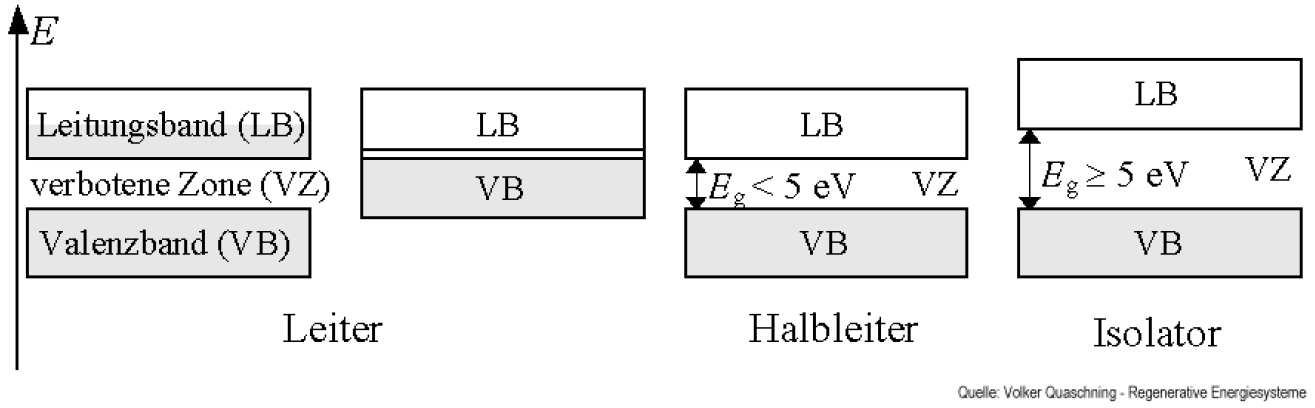
\includegraphics[width=0.5\textwidth]{images/Leitungsband} \\ \columnbreak 
\ \\ \vfill \columnbreak 
Mit der Energie des Lichtes kann ein Elektron auf eine höhere Bahn gehoben werden oder auch herausgeschlagen werden. \\ 
$E = \frac{h * c}{\lambda}$
\end{multicols}

\begin{multicols}{2}
\subsection{Photometrie}
\subsubsection{Empfindlichkeit des Auges}
Bei einer Wellenlänge von 555 nm, einer gelb-grünen Spektralfarbe entsprechend, ist das Auge am empfindlichsten. Bei etwa 510 nm (grün) auf der einen Seite, und bei etwa 610 nm (orangerot) auf der anderen Seite des Maximums erreicht das Auge nur noch die halbe Empfindlichkeit. Bei 665 nm, der Farbe typischer roter Leuchtdioden, beträgt die Empfindlichkeit nur 4,5 Prozent derjenigen bei 555 nm. Bei etwa 380 nm (violett) bzw. 780 nm (tiefrot) ist die Empfindlichkeit fast Null. \\ \\

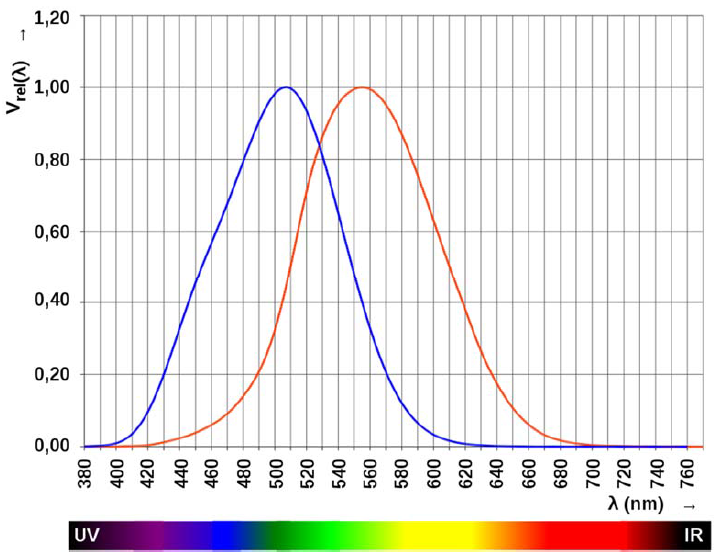
\includegraphics[width=0.4\textwidth]{images/empfindlichkeit_auge} 
\end{multicols}

\subsubsection{Übersicht}
\begin{tabular}{|l|l|l|l|l|l|}
    \hline
    \multicolumn{3}{|l|}{Strahlungsphysikalische Grössen} & \multicolumn{3}{l|}{Lichttechnische Grössen} \\ \hline
    Grösse             & Symbol   & Einheit          & Grösse             & Symbol & Einheit      \\ \hline
    Strahlungsstrom    & $\Phi_e$ & $W$              & Lichtstrom         & $\Phi_v$ & $lm$       \\ \hline
    Strahlstärke       & $I_e$    & $Wsr^{-1}$       & Lichtstärke        & $I_v$    & $cd$       \\ \hline
    Strahldichte       & $L_e$    & $Wm^{-2}sr^{-1}$ & Leuchtdichte       & $L_v$    & $cdm^{-2}$ \\ \hline
    Bestrahlungsstärke & $E_e$    & $Wm^{-2}$        & Beleuchtungsstärke & $E_v$    & $lx$       \\ \hline
\end{tabular}
\section{Photonik Aktoren}
\subsection{Lichtquellen}
\subsubsection{Temperaturstrahler}
\begin{multicols}{2}
    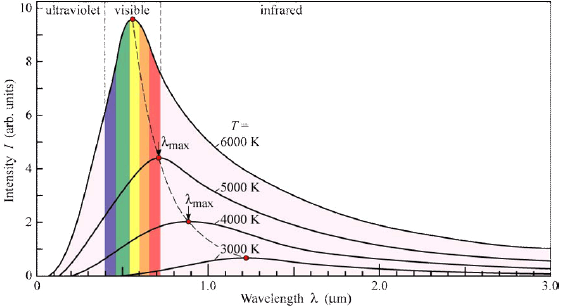
\includegraphics[width=0.5\textwidth]{images/temperaturstrahler} \vfill \columnbreak
    Die Temperaturstrahler können in zwei kategorien eingeteilt werden:
    \begin{compactitem}
        \item Natürliche Temperaturstrahler: Sterne, Blitze, Feuer, ...
        \item Künstliche Temperaturstrahler: Kerzen, Glühbirnen, ... 
    \end{compactitem}
    Jeder Körper mit Temperatur wärmer als der absolute Nullpunkt gibt elektromagnetische Strahlung ab.
    Die Temperatur bestimmt dabei die Lichtintensität: $I=\sigma*T^4$
\end{multicols}

\subsection{Die Sonne}
\subsubsection{Sonneneinstrahlung}
Der Bezugswert der Sonneneinstrahlung für die Erde ist mit der Solarkonstante festgelegt. Sie hat den Wert $1.37 \frac{kW}{m^2}$ für senkrecht zur Probefläche einfallendes Licht ohne atmosphärische Einflüsse, also ausserhalb der Atmosphäre. Dieser Wert gilt damit für die Verhältnisse im Weltraum. Bei unbedecktem Himmel, trockener Luft und am Erdboden ist der Wert der sogenannten terrestrischen Solarkonstante $1 \frac{kW}{m^2}$. Als Vergleich zur Stärke der Sonneneinstrahlung kann man eine kleine Herdplatte heranziehen. Ihre Leistung liegt - auf höchster Stufe - bei etwa einem Kilowatt, ihre Fläche (18cm Durchmesser) bei etwa 0.025m, die Leistung pro Fläche $40 \frac{kW}{m^2}$.

\subsubsection{Airmass AM}
Das Airmass ist ein Mass dafür, wie lang der Weg des Lichts durch die Atmosphäre ist.

\subsection{Glühlampe}
In einer Glühlampe fliesst ein elektrischer Strom durch einen dünnen Leiter, z.B. ein Metall-Faden aus Wolfram. Fliesst ein ausreichend starker elektrischer Strom wird dieser erhitzt, so dass er glüht. Die Temperatur der Glühwendel beträgt je nach Bauform ca. $1500$ – $3000^\degree C$, so dass sie gemäss dem planckschen Strahlungsgesetz elektromagnetische Strahlung emittiert. Die Strahlung liegt vor allem im Bereich der Infrarotstrahlung und nur wenig (\textless5\%) im Bereich des sichtbaren Lichts.

\subsection{Lumineszenz-Strahler}
Unterbegriffe der Lumineszenz sind Fluoreszenz (kurzes Nachleuchten) und Phosphoreszenz (langes Nachleuchten). Es gibt auch hier zwei Varianten:
\begin{compactitem}
    \item Biologische Lumineszenz-Strahler sind Glühwürmchen
    \item Chemische Lumineszenz-Strahler sind z.B. Leuchtstäbe
\end{compactitem}
Strahlung kann abgegeben werden (Lumineszenz) oder aufgenommen werden (Photoeffekt) nach dem Gesetz: $\Delta E = h*v$ wobei $h = 6.6*10^{-34} \frac{J}{Hz}$

\subsection{Leuchtdioden (Light Emitting Diode)}
\subsubsection{Funktionsweise}
\begin{wrapfigure}{r}{0.25\textwidth}
    \centering
    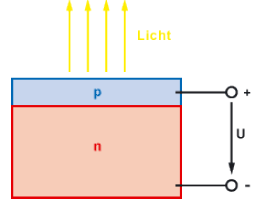
\includegraphics[width=0.22\textwidth]{images/LED}
\end{wrapfigure}
Eine Leuchtdiode besteht aus einem n-leitenden Grundhalbleiter. Darauf ist eine sehr dünne p-leitende Halbleiterschicht mit grosser Löcherdichte aufgebracht. Wie bei der normalen Diode wird die Grenzschicht mit freien Ladungsträgern überschwemmt. Die Elektronen rekombinieren mit den Löchern. Dabei geben die Elektronen ihre Energie in Form eines Lichtblitzes frei. Da die p-Schicht sehr dünn ist, kann das Licht entweichen. Da von dem Halbleiterkristall nur eine geringe Lichtstrahlung ausgeht, ist das Metall unter dem Kristall halbkugelförmig. Dadurch wird das Licht gestreut. Durch das linsenförmige Gehäuse wird das Licht gebündelt. So können Leuchtdioden schon mit wenigen milliampere Strom sehr hell leuchten.

\subsubsection{Farben und Materialien}
\begin{wrapfigure}[4]{l}{0.5\textwidth}
    \vspace{-12pt}
    \centering
    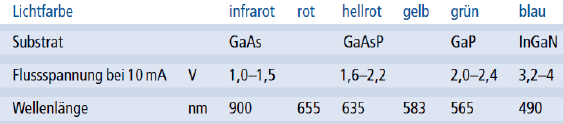
\includegraphics[width=0.48\textwidth]{images/kennwert_LED}
\end{wrapfigure}
Die Farbe des Lichts bzw. die Wellenlänge des Lichts wird vom Halbleiterkristall und von der Dotierung bestimmt. \\

\subsection{Laser (Light Amplification by Stimulated Emission of Radiation)}
\begin{wrapfigure}[7]{l}{0.5\textwidth}
    \vspace{-12pt}
    \centering
    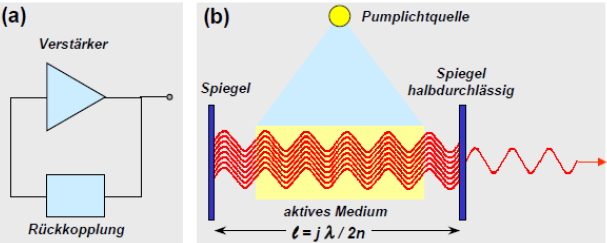
\includegraphics[width=0.48\textwidth]{images/laser}
\end{wrapfigure}
Der Laser ist eine monochrome, kohärente, polarisierte Lichtquelle mit hoher Intensität und scharfer Bündelung des Strahls. Es gibt dabei drei verschiedene Arten: Gas-, Farbstoff-, Halbleiterlaser.

\subsubsection{Funktionsweise}
Der Laser ist ein Resonator zwischen 2 Spiegeln, das Licht tritt an halbdurchlässigem Spiegel aus.

\subsubsection{Laserdiode}
\begin{wrapfigure}[4]{l}{0.25\textwidth}
    \vspace{-12pt}
    \centering
    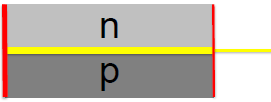
\includegraphics[width=0.22\textwidth]{images/laserdiode}
\end{wrapfigure}
Die Laserdiode hat pn-Übergang und zwei spiegelnde Flächen. Es erfolgt eine stimulierte Emission (bei LED spontane Emission). Ein einfallendes Photon regt dabei ein zweites Photon an. Dieses besitzt exakt dieselben Eigenschaften (Wellenlänge, Ausbreitungsrichtung und Polarisation). Erst ab Schwellstrom ($I_{th}$)funktioniert die Diode als Laser, sonst ist es nur eine LED! Die Laserdioden werden auf Wafern hergestellt. Die Wafer werden geschnitten. Danach müssen die Schnittflächen verspiegelt werden. 

\subsubsection{Laserdiode VCSEL}
\begin{wrapfigure}[6]{l}{0.25\textwidth}
    \vspace{-12pt}
    \centering
    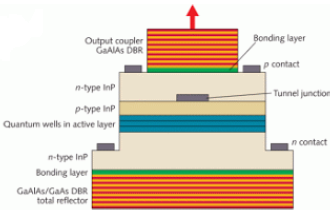
\includegraphics[width=0.22\textwidth]{images/vcsel}
\end{wrapfigure}
Bei VCSEL (Vertical Cavity Surface Emitting Laser) werden die spiegelnden Flächen auf dem Wafer abgeschieden. Viele Schichten aus Materialien mit unterschiedlichem Brechungsindex ergeben dabei einen Interferenzfilter, welcher die gewünschte Wellenlänge spiegelt. Der Aufbau ist komplex, aber es lassen sich zehntausende Laser auf einem Wafer gleichzeitig herstellen. VCSEL sind somit deutlich billiger als normale Laserdioden.





\section{Photonik Sensoren}
\subsection{Helligkeits-Sensoren}
\subsubsection{Fotowiderstände LDR (Light Dependent Resistor)}
Trifft Licht auf die fotoempfindliche Fläche des Fotowiderstands, verringert sich der Widerstand durch den inneren fotoelektrischen Effekt. D.h. ein eintreffendes Photon hebt ein Elektron in das Leitungsband, welches sich nun frei im Kristall bewegen kann: Das Material wird niederohmiger. LDR's haben den Nachteil, dass sie ziemlich wärmeempfindlich und träge sind (Der Dunkelwiderstand wird erst nach $\frac{1}{60}s$ wieder erreicht).

\subsubsection{Photodiode}
\begin{wrapfigure}[14]{l}{0.5\textwidth}
    %\vspace{-12pt}
    \centering
    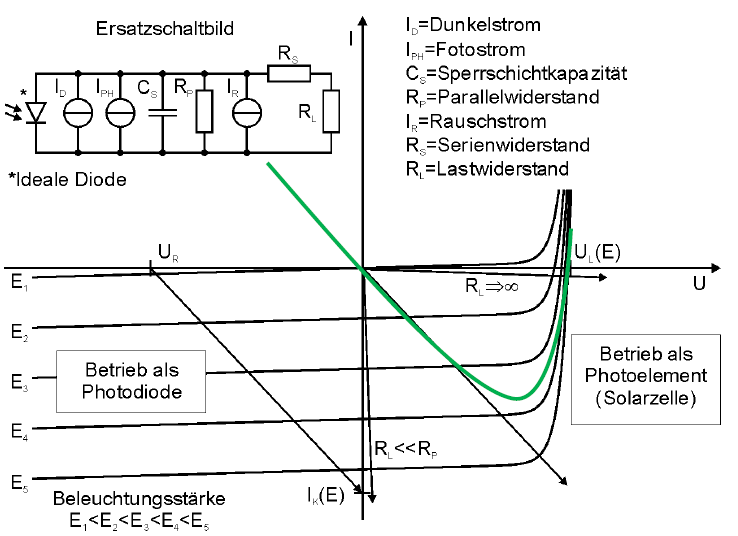
\includegraphics[width=0.42\textwidth]{images/photodiode}
\end{wrapfigure}
Treffen Photonen mit ausreichender Energie auf einen pn-Übergang, so werden Ladungsträger (Elektron-Loch-Paare) erzeugt. In der Raumladungszone driften die Ladungsträger schnell entgegen der Diffusionsspannung in die gleichartig dotierten Zonen, und führen zu einem Strom. Ohne externe Verbindung der Anschlüsse entsteht an diesen eine messbare Spannung gleicher Polarität wie die Durchflussspannung (Sättigung). Sind die Anschlüsse miteinander elektrisch verbunden oder befinden sie sich an einer Spannung in Sperrrichtung der Diode, fliesst ein Photostrom, der proportional zum Lichteinfall ist. Die Photonen müssen eine höhere Energie als die des Bandabstandes aufweisen, um diesen Effekt hervorzurufen.

\subsection{Solarzellen}
Eine Photodiode kann als Solarzelle betrieben werden. Dabei gibt es die folgenden Betriebsmodi:
\begin{compactitem}
    \item ohne Last: Sättigung mit Leerlaufspannung $U_L$, $U_L$ hängt dabei wenig von der Lichtstärke ab
    \item mit niederohmiger Last: Bei kleinerem $R_L$ sinkt Spannung und Strom steigt (bis max. Kurzschlussstrom $I_K$)
    \item bei MPP: Am Knick der Kennlinie liegt der angestrebte Arbeitspunkt MPP (Maximum Power Point) mit max. Leistung. Der MPP liegt dabei bei ca. 80\% Leerlaufspannung.
\end{compactitem}

\subsection{Photodiode als Lichtsensor}
\subsubsection{Betrieb im Quasi-Kurzschluss (U = 0)}
\begin{wrapfigure}[5]{l}{0.25\textwidth}
    %\vspace{-12pt}
    \centering
    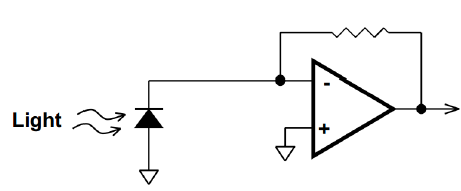
\includegraphics[width=0.22\textwidth]{images/photodiode_betrieb_01}
\end{wrapfigure}
Der Photo-Strom wird in Sperrrichtung erzeugt und ist linear abhängig von der Bestrahlungsstärke. Der Opamp ist als Transimpedanzverstärker geschaltet. Es erfolgt keine Änderung der Spannung und keine Umladung von Kapazitäten. Dadurch ist die Schaltung relativ schnell. Die grosse Diodenkapazität ist aber ein Problem für den Opamp. 

\subsubsection{Betrieb im Sperrbereich}
\begin{wrapfigure}[4]{l}{0.25\textwidth}
    %\vspace{-12pt}
    \centering
    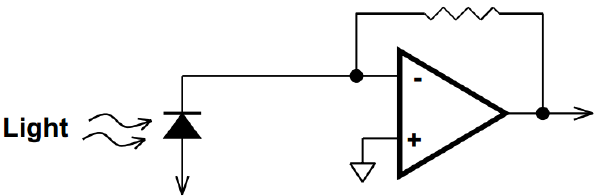
\includegraphics[width=0.22\textwidth]{images/photodiode_betrieb_02}
\end{wrapfigure}
Es liegt eine negative Spannung über der Photodiode. Die Diodenkapazität ist dadurch kleiner und die Schaltung schneller. Der Dunkelstrom $I_D$ steigt hingegen mit Spannung und Temperatur an. Er überlagert den Photostrom und bestimmt das Rauschen.

\subsection{Phototransistor}
Phototransistoren sind wesentlich empfindlicher als Photodioden, die Basis-Emitter-Diode ist eine Photodiode. Der Photostrom wird verstärkt mit dem Stromverstärkungsfaktor $\beta$. Allerdings sind sie viel langsamer als Photodioden.

\subsection{Spektrale Empfindlichkeit}
Silizium ist am empfindlichsten bei ca. 850nm, wird aber für gesamtes Spektrum von blau bis NIR (400nm – 900nm) genutzt. Andere Wellenlängen bedingen aufwändigere Herstellungsprozesse mit zusätzlichen Dotierungen.

\subsubsection{Eindringtiefe der Photonen}
Je nach Wellenlänge dringt das Licht mehr oder weniger tief ins Halbleitermaterial ein. Bei Silizium ergeben sich z.B. folgende Eindringtiefen:
\begin{compactitem}
    \item blau, $400nm$: $a = 2*10^4cm^{-1}$ $\rightarrow$ $d=500nm$
    \item rot, $700nm$: $a = 5*10^3cm^{-1}$ $\rightarrow$ $d=2um$
    \item infrarot, $1000nm$: $a = 3*10^2cm^{-1}$ $\rightarrow$ $d=33um$
\end{compactitem}

\subsubsection{CMOS-IC-Prozesse mit Fotodioden}
\begin{multicols}{4}
    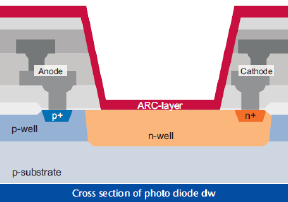
\includegraphics[width=0.24\textwidth]{images/eindringtiefe_01}
    Standard Diode in jedem Prozess vorhanden, maximum bei Rot \\
    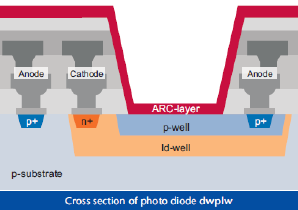
\includegraphics[width=0.24\textwidth]{images/eindringtiefe_02}
    Zweite Diode näher an der Si-Oberfläche, bessere Blau-Empfindlichkeit \\
    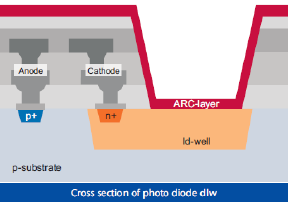
\includegraphics[width=0.24\textwidth]{images/eindringtiefe_03}
    Low-doped NWell: Depletionszone tiefer im Substrat, mehr IR-Empfindlichkeit \\
    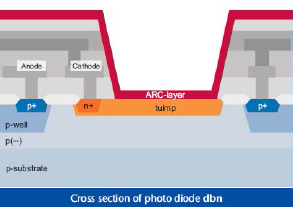
\includegraphics[width=0.24\textwidth]{images/eindringtiefe_04}
    Sehr dünne, oberflächennahe Implantierung, Blau-und UV-Empfindlich (DVD, Blueray-Empfänger)
\end{multicols}

Für kürzere Wellenlängen (UV+Röntgen) wird ein Scintillator-Kristall(z.B. CäsiumIodidCsI) auf die Diode aufgebracht: Die Strahlung regt den Kristall an, welcher dann bei einer längeren Wellenlänge im sichtbaren Bereich leuchtet.

\subsection{Avalanche-Photodioden}
\begin{wrapfigure}[11]{l}{0.35\textwidth}
    %\vspace{-12pt}
    \centering
    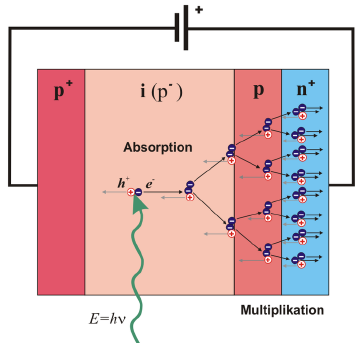
\includegraphics[width=0.25\textwidth]{images/apd}
\end{wrapfigure}
Avalanche-Photodioden sind hochempfindlich und schnell. Sie nutzen den inneren photoelektrischen Effekt zur Ladungsträgererzeugung und den Lawinendurchbruch (Avalanche-Effekt) zur internen Verstärkung. Eine Detektierung von sehr geringer Strahlung ist möglich (bis hin zu einzelnen Photonen). Die spektrale Empfindlichkeit liegt je nach verwendetem Material in einem Bereich von ca. 250 – 1700nm.
\subsubsection{Aufbau}
Photonen werden in der vollständig verarmten intrinsischen i-Schicht absorbiert und erzeugen dort Ladungsträgerpaare. In einer Si-APD werden die Elektronen zur Multiplikationszone hin beschleunigt und verursachen dort die Ladungslawine.

\subsection{CCD (Charge-Coupled-Device)}
\subsubsection{Funktionsweise}
\begin{multicols}{3}
    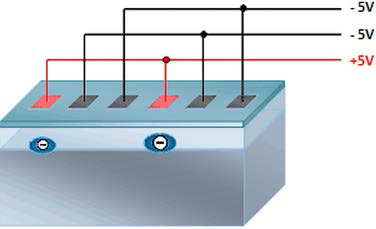
\includegraphics[width=0.32\textwidth]{images/ccd_01}
    Elektronen werden angezogen unter (rote) Elektroden mit pos. Spannung \\
    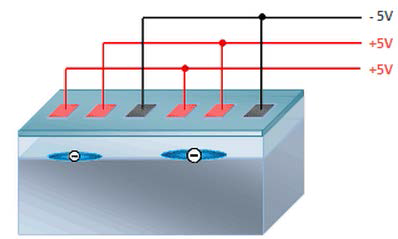
\includegraphics[width=0.32\textwidth]{images/ccd_02}
    Benachbarte Elektroden aktiviert: Elektronen verteilen sich unter 2 Elektroden \\
    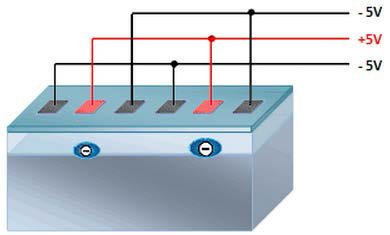
\includegraphics[width=0.32\textwidth]{images/ccd_03}
    Linke Elektrode deaktiviert, Elektronen sammeln sich unter nächster Elektrode \\
\end{multicols}
\begin{multicols}{3}
    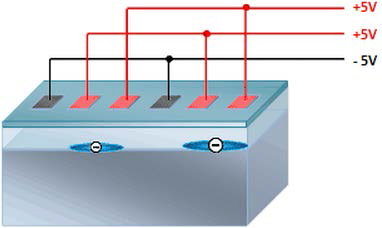
\includegraphics[width=0.32\textwidth]{images/ccd_04}
    Benachbarte Elektroden aktiviert, Elektronen verteilen sich wieder unter 2 Elektroden \\
    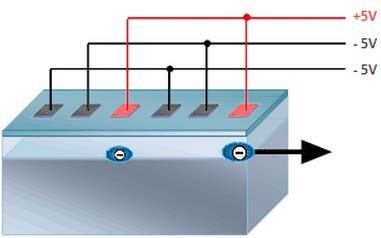
\includegraphics[width=0.32\textwidth]{images/ccd_05}
    Elektronen sind am Rand des Schieberegisters, Weiterverarbeitung mit Ladungsverstärker, ADC \\
    Die Frequenz, wie oft der Sensor pro Sekunde der in der Lage ist, die Ladung um einen Pixel weiter zu transportieren, wird "Pixel clock" genannt. Die Frequenzen, mit den CCDs heute betrieben werden, betragen rund 25 bis 50 MHz. \\ \ \\ \ \\ \ \\
\end{multicols}

\subsubsection{Auslesevarianten}
\begin{multicols}{2}
    \paragraph{Interline Transfer Sensor}
    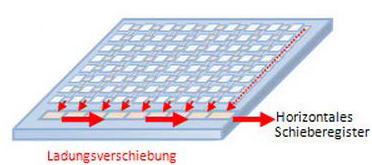
\includegraphics[width=0.39\textwidth]{images/ccd_interline} \\
    Bei dieser Variante erfolgt eine Trennung von Pixel und Speicherzellen. Der fillfactor des Sensors beträgt nur etwa 30 Prozent. Mikrolinsen helfen aber die Lichtausbeute zu erhöhen.
    
    \paragraph{Fullframe Transfer Sensor}
    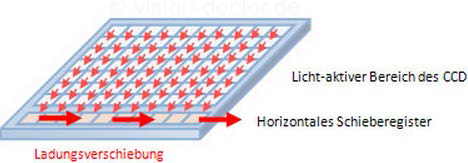
\includegraphics[width=0.49\textwidth]{images/ccd_fullframe}
    Die komplette Sensorfläche ist lichtaktiv. Er ist ideal für eine maximale Helligkeitsempfindlichkeit und er besitzt keine vertikalen Schieberegister. 
\end{multicols}

\subsubsection{Farb-Filter}
\begin{wrapfigure}[7]{l}{0.25\textwidth}
    %\vspace{-12pt}
    \centering
    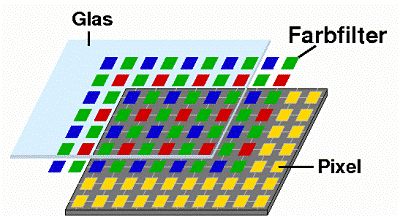
\includegraphics[width=0.24\textwidth]{images/ccd_filter}
\end{wrapfigure}
Die meisten Sensoren werden mit einem optischen Filter betrieben. Ein oft eingesetzter Filter basiert auf dem Bayer-Pattern. Dieses enthält 50\% grüne, 25\% blaue und 25\% rote Farbfilter. Ein De-Mosaicing ist anschliessend noch nötig. \\
In einer Alternativlösung wird anstelle eines Filters die unterschiedliche Eindringtiefe von Licht mit unterschiedlicher Wellenlänge ausgenutzt. Dabei besteht ein Pixel aus 3 gestackten Fotodioden. Dabei geht kein Licht verloren, die Separation ist aber schlecht.

\subsection{CMOS-Bildsensoren}
\subsubsection{Active Pixel Sensor (APS)}
\begin{wrapfigure}[15]{l}{0.25\textwidth}
    %\vspace{-12pt}
    \centering
    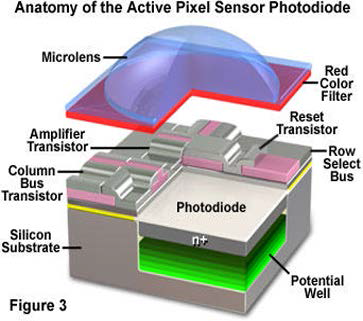
\includegraphics[width=0.24\textwidth]{images/cmos_aps}
    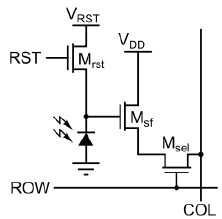
\includegraphics[width=0.15\textwidth]{images/cmos_aps_aufbau}
\end{wrapfigure}
Die Umwandlung von Ladung in Spannung geschieht innerhalb des Pixels. Jedes Pixel hat deshalb seine eigene Auslese-Elektronik. Dadurch ist ein flexibles auslesen (Region-of-Interest (ROI)) möglich. 
\paragraph{Funktionsweise}
Eine Zelle besteht aus einer Photodiode und 3 NMOS-Transistoren. Die Photodiode wird im Reset auf eine hohe Spannung gesetzt. Der Photostrom entlädt die Diodenkapazität, dies führt zu einer Integration des Photostromes während der Integrationszeit. Der Source-Follower-Transistor ($M_{sf}$) folgt der Diodenspannung (verschoben um konstante Spannung $V_{TH}$). Nach der Integrationszeit wird die Spannung am Pixel über den Source-Follower gemessen und über $M_{sel}$ ausgelesen. Jeweils eine ganze Zeile wird mit dem Reset-Transistor zurückgesetzt. Mit dem Selekt-Transistor wird eine einzelne Zeile aus dem Bildfeld angewählt. Jede Ausgangskolonne hat einen eigenen Kolonnen-Verstärker. Teilweise wandeln Kolonnen-ADC's das Signal direkt in ein digitales Signal um. Ein Kolonnenmultiplexer selektiert am Schluss eine Kolonne nach der anderen und gibt das Signal an den Ausgang aus. \\

\paragraph{Global Shutter Pixel}
Bei einem Rolling Shutter Pixel werden sich schnell bewegende Objekte falsch aufgenommen. Aus diesem Grund gibt es Global Shutter Pixel. Diese haben einen zusätzlichen Sense-Node (SN). Bei dieser Art werden alle Pixel gleichzeitig zurückgesetzt und die integrierte Ladung aller Pixel werden gleichzeitig auf den Sense-Node übertragen. Dabei integrieren alle Pixel über den exakt selben Zeitraum, die Bewegungen werden eingefroren. Ein Nachteil ist, dass die Photodiode kleiner wird bei gleichbleibender Pixelfläche.

\newpage
\paragraph{Rauschen im Pixel}
\begin{wrapfigure}[15]{r}{0.45\textwidth}
    %\vspace{-12pt}
    \centering
    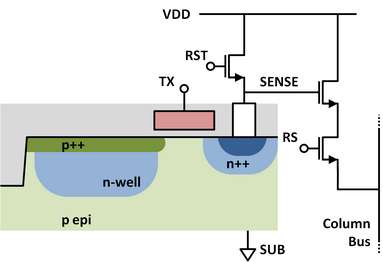
\includegraphics[width=0.42\textwidth]{images/cmos_aps_pinned}
\end{wrapfigure}
Wird ein Knoten über einen Transistor auf ein Potential gesetzt und der Transistor danach geöffnet, so ist das Potential auf dem Knoten rauschbehaftet. Die Rauschspannung kann dabei folgendermassen berechnet werden: $V_{n, kTC} = \sqrt{\frac{kT}{C}}$. Die Anzahl der Rauschelektronen kann ebenfalls bestimmt werden: $n_{n, kTC} = \frac{\sqrt{kT*C}}{q}$ \\
Dies kann verhindert werden indem durch einen zusätzlichen Layer $p++$ die Photodiode gepinnt wird. Dabei ist die Photodiode vom Ausleseknoten über das Gate TX getrennt. Wird TX auf high gesetzt, fliesst alle Ladung in den Ausleseknoten. Dies erlaubt Correlated Double Sampling (CDS) und eliminiert das Reset-oder $\frac{kT}{C}$-Rauschen.
\\
\begin{multicols}{2}
    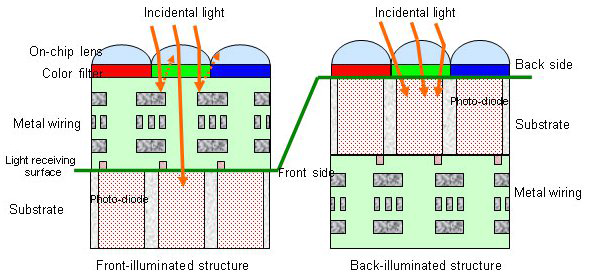
\includegraphics[width=0.48\textwidth]{images/cmos_iluminated} 
    \paragraph{Front- und Back-illuminated CMOS}
    \begin{compactitem}
        \item Front-illuminated Sensoren: Metall-Verbindungen absorbieren Licht 
        \item Back-illuminated Sensoren: Höhere Lichtausbeute
    \end{compactitem}
\end{multicols}



\section{Photonik Anwendungen}
\subsection{Lichtschranken}
\begin{multicols}{3}
    \subsubsection{Einweg-Lichtschranke}
    \begin{compactitem}
        \item Sender und Empfänger stehen sich gegenüber
        \item 1 Modul: Gabellichtschranke (z.B.: Drehzahlmesser)
        \item Sender und Empfänger getrennt: Justierung nötig
        \item Detektiert Unterbruch
    \end{compactitem}
    
    \subsubsection{Reflex-Lichtschranke}
    \begin{compactitem}
        \item Sender und Empfänger im selben Gehäuse: nur ein Kabel nötig
        \item Am anderen Ende Reflexfolie / Retroreflektor (Katzenauge)
        \item Detektiert Unterbruch
    \end{compactitem}
    
    \subsubsection{Reflex-Lichttaster}
    \begin{compactitem}
        \item Kein Reflektor: Normalerweise kommt kein Licht zurück
        \item Nahes Objekt reflektiert genügend Licht: Detektion
        \item Von Objekteigenschaften abhängig!
    \end{compactitem}
\end{multicols}

\subsubsection{Nachteile}
\begin{compactitem}
    \item Fremdlicht kann die Funktion der Lichtschranke beeinflussen
    \item Möglichkeiten der Unterdrückung
    \begin{compactitem}
        \item Optischer Filter: nur das Licht, dass ausgesandt wird, gelangt zum Detektor, Fremdlicht mit anderem Spektrum wird unterdrückt
        \item Mehr Leistung: Optik, LED zu Laser, Verhältnis Nutz- zu Fremdlicht verbessert sich
        \item Moduliertes Licht: Mit elektrischem Filter wird die Modulationsfrequenz herausgesucht
    \end{compactitem}
\end{compactitem}

\begin{multicols}{2}
    \subsection{Ambientlight Sensor (ALS)}
    \begin{compactitem}
        \item Detektiert die Umgebungshelligkeit zum Dimmen des Displays
        \item Ist oftmals eine Photodiode
        \item Meist im Proximity-Sensor eingebaut
        \item Teils mit RGB-Farbdetektion
    \end{compactitem}
    
    \subsection{Proximity-Sensor}
    \begin{compactitem}
        \item kleiner Reflexlichttaster
        \item Unterschiedliche Reflexion von heller/dunkler Haut und blondem/schwarzem Haar sowie Schmutz auf dem Glas können Probleme verursachen.
    \end{compactitem}
\end{multicols}

\subsection{Optische Distanzmessung}
\subsubsection{Vergleich}
\begin{multicols}{4}
    \paragraph{Stereo}
    \begin{compactitem}
        \item Passive Messung
        \item Objektstruktur nötig, Abschattungen möglich
        \item Rechenaufwändig
    \end{compactitem}
    
    \paragraph{Laufzeitmessung (Time-of-Flight)}
    \begin{compactitem}
        \item Aktive Beleuchtung nötig
        \item Keine Abschattung
    \end{compactitem}
    \ \\
    
    \paragraph{Triangulation}
    \begin{compactitem}
        \item Aktive Beleuchtung nötig
        \item Keine Struktur nötig
        \item Relativ einfache Berechnung
    \end{compactitem}
    \ \\
    
    \paragraph{Interferometrie}
    \begin{compactitem}
        \item Höchste Auflösung
        \item Aufwändige Technik
    \end{compactitem}
    \ \\ \ \\ \ \\
\end{multicols}

\newpage
\subsubsection{Stereo Messung}
\begin{wrapfigure}[6]{l}{0.3\textwidth}
    %\vspace{-12pt}
    \centering
    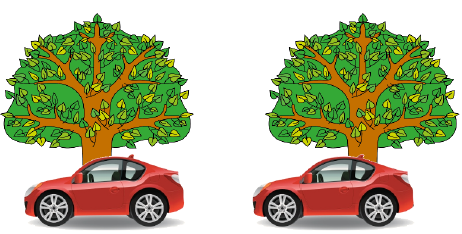
\includegraphics[width=0.25\textwidth]{images/photonik_anwendung_stereo}
\end{wrapfigure}
\ 
\vspace{-5pt}
\begin{compactitem}
    \item Diese Methode ist dem menschlichen Sehen nachempfunden.
    \item Es ist ein passives System: keine Beleuchtung nötig.
    \item Eine aufwändige Berechnung ist notwendig (Kreuzkorrelation zwischen den Bildern muss berechnet werden).
    \item Einfarbige Flächen können nicht bestimmt werden.
\end{compactitem}

\subsubsection{Triangulations Messung}
\begin{wrapfigure}[4]{l}{0.3\textwidth}
    %\vspace{-12pt}
    \centering
    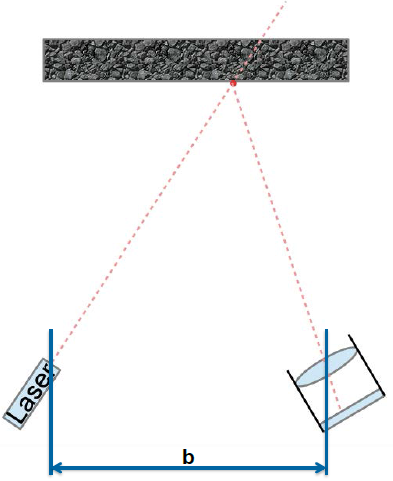
\includegraphics[width=0.1\textwidth, angle=90]{images/photonik_anwendung_triangulation}
\end{wrapfigure}
\ 
\vspace{-5pt}
\begin{compactitem}
    \item Ein Zeilensensor misst den Fokus des reflektierten Laserlichts.
    \item Mit der Winkelbeziehung wird die Distanz bestimmt.
    \item Eine Beleuchtung ist nötig.
    \item Einfache Detektion und Berechnung der Distanz über die Geometrie.
\end{compactitem}

\subsubsection{Time-of-Flight Messung}
\begin{compactitem}
    \item Ein perfekter Puls kann nicht generiert werden.
    \item Die Modulation einer Lichtquelle mit Sinussignal ist eine Alternative. 
    \item Es wird dann der Phasenunterschied vom ausgesendeten zu empfangenen Signal gemessen.
    \item Nachteil: Nicht ein-eindeutige Position, Auflösung nur innerhalb einer Periode möglich
\end{compactitem}

\paragraph{Funktionsweise}
\begin{wrapfigure}[4]{l}{0.3\textwidth}
    %\vspace{-12pt}
    \centering
    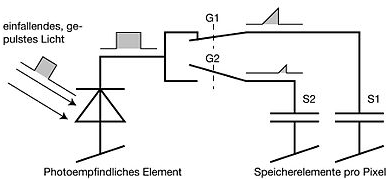
\includegraphics[width=0.29\textwidth]{images/tof_fkt_01}
    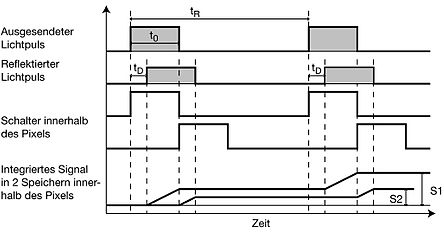
\includegraphics[width=0.29\textwidth]{images/tof_fkt_02}
\end{wrapfigure}
\ 
\vspace{-5pt}
\begin{compactenum}
    \item Puls-Signal wird ausgesendet.
    \item Licht des Sensors wird abwechselnd auf 2 Kapazitäten geschaltet
    \item Je nach Verzögerung ist die Verteilung der Photonen anders.
    \item Es liegen somit andere Spannungen an S1 und S2.
    \item Daraus kann ein Rückschluss auf Eintreff-Zeit des Pulses gemacht werden.
    \item Verschiebt sich die Ankunft des Pulses, so verändern sich Anteile die S1 und S2.
    \item Daraus kann die Distanz berechnet werden. \\
\end{compactenum}

\ \\
\subsection{Optische Datenübertragung}
\subsubsection{Vorteile}
\begin{compactitem}
    \item Licht anstelle eines elektrischen Signals als Übertragungsmedium
    \item Störungsarm: kein elektrisches Einkoppeln, kein Übersprechen, keine Potentialprobleme
    \item Kleine Dämpfung, grosse Reichweite
    \item Grosse Bandbreite: $>$ 100Gbit/s
\end{compactitem}

\subsubsection{Glasfaserarten}
\begin{wrapfigure}[14]{l}{0.6\textwidth}
    %\vspace{-12pt}
    \centering
    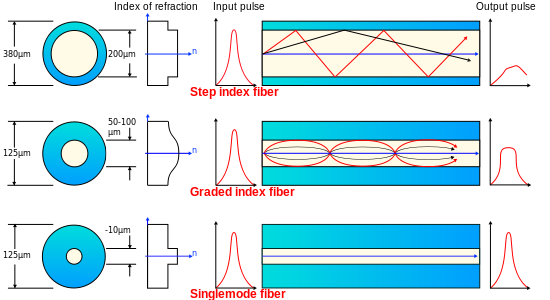
\includegraphics[width=0.55\textwidth]{images/glasfaserarten}
\end{wrapfigure}
\ 
\vspace{-5pt}
\begin{compactitem}
    \item POF: (polymericopticalfibre), Kunststoff, \\
    Ø = 1mm, billig, Kopplung an LED, \\
    kleine Datenrate $<$100MB/s, kurze Verbindung
    \item Multimode (Mantel orange, türkis), \\
    Ø = 50$\mu$m/62.5$\mu$m, \\
    hohe Datenrate
    \item Monomode(gelb), \\
    Ø $<$10$\mu$m, \\
    höchste Datenrate
\end{compactitem}
\ \\

\subsubsection{Glasfaser als Sensor}
\begin{multicols}{2}
    \paragraph{Faserkreisel}
    \begin{compactitem}
        \item Bei Ruhe: Lichtwege sind identisch, konstruktive Interferenz
        \item Bei Drehung: der eine Lichtweg wird etwas kürzer, der andere länger, destruktive Interferenz, resp. das Linienmuster verschiebt sich
    \end{compactitem}
    
    \paragraph{Faseroptische Druck-und Temperatursensoren}
    \begin{compactitem}
        \item Durch Druck oder Temperatur ändert sich die (Raman-) Reflexionan dieser Stelle, örtlich aufgelöste Messung
        \item Wird eingesetzt bei Staumauern, Flugzeugflügel, ...
        \item Einfacher Sensor, «aber teure Auswertung
    \end{compactitem}
\end{multicols}

\subsection{Kontaktlose Temperaturmessung mittels Infrarotstrahlung}
\subsubsection{Seebeck-Effekt}
\begin{compactitem}
    \item Der Seebeck-Effekt tritt auf bei Temperaturdifferenzen in Leitern.
    \item Am warmen Ende eines Leiters haben Elektronen mehr Energie als am kalten Ende.
    \item Die Beweglichkeit der Elektronen ist grösser.
    \item Durch Diffusion bewegen sich mehr energiereiche Elektronen zum kalten Ende als energiearme Elektronen in die entgegengesetzte Richtung.
    \item Durch diese Thermodiffusionsströme entsteht zwischen den Kontaktstellen eine elektrische Spannung, die Thermo- oder Seebeck-Spannung.
\end{compactitem}


\begin{minipage}{0.45\textwidth}
       \begin{equation*} 
        \begin{split} 
          &V_{out}=N \cdot S \cdot(T_x - T_{REF})\\
          &\text{N: Number of thermocouples}\\
          &\text{S: Seebeck coefficient}
        \end{split} 
      \end{equation*}

\end{minipage}
\begin{minipage}{0.5\textwidth} 
    \vspace{-0.5cm}
    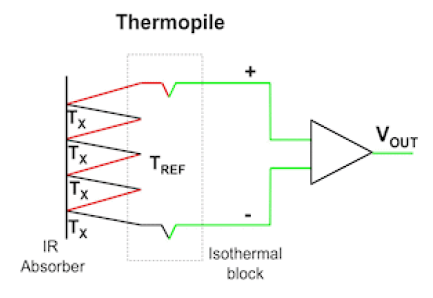
\includegraphics[width=1\textwidth]{images/Thermo}
\end{minipage}


\input{sections/highspeed_electronics}
\newpage
\section {Oszillatoren}
\subsection {Definition und Klassifikation von Oszillatoren} 
\raggedright

\begin{multicols}{2}
    Oszillatoren werden in zwei Hauptgruppen unterteilt:
    \begin{compactitem}
        \item \textbf{Abgestimmte} Oszillatoren aus einem Verstärker und einem Frequenz bestimmenden Newtzwerk, die in \textbf{positiver} Rückkopplung betrieben werden.
        \item \textbf{Nichtabgestimmte} oder schaltende Oszillatoren bestehen dagegen aus einem Schaltelement mit mindestens zwei stabilen Zuständen (\textbf{Multivibrator}) und einem Integrator oder Tiefpassfilter, welches zwischen den Zuständen des Schaltelementes umgeladen wird. Die Umladezeit des Integrators ist hier Frequenz bestimmend während die Amplitude üblicherweise durch die Pegel des Schaltelementes gegeben ist.
    \end{compactitem}
    
    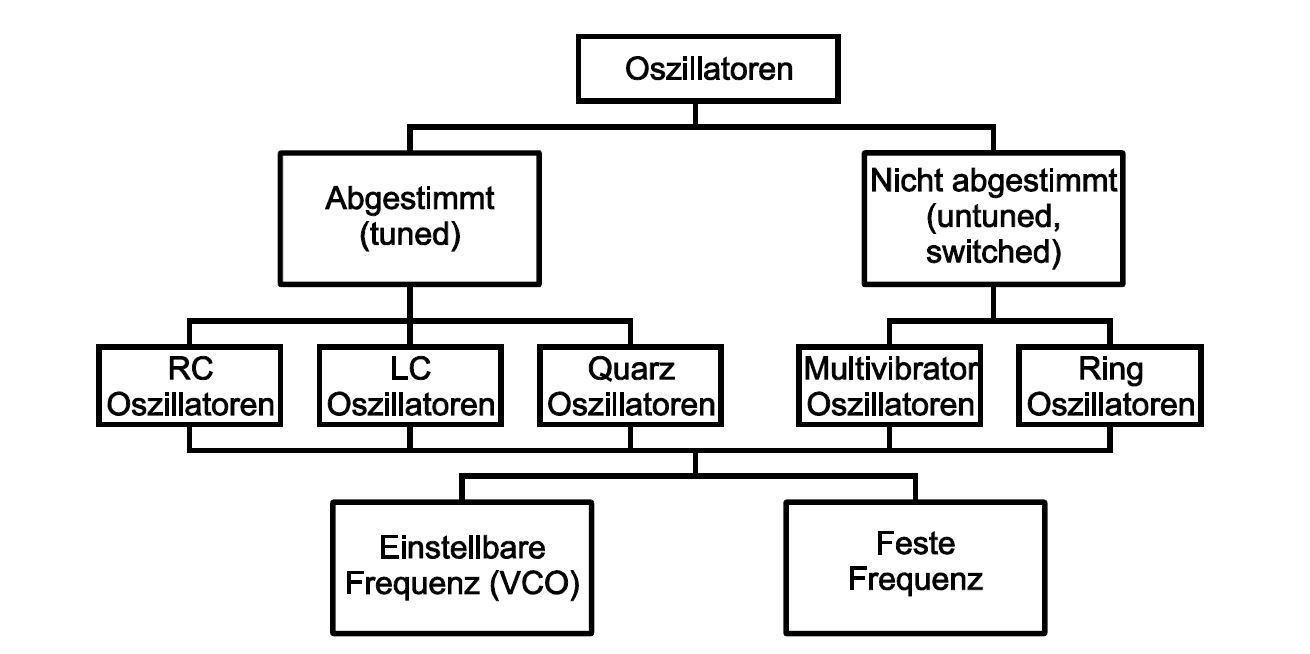
\includegraphics[width=0.54\textwidth]{images/Klassifikation_Oszillatortypen}
    \ \\ \ \\ \ \\ \ \\
\end{multicols}

\FloatBarrier
\subsection{Oszillatorgrundprinzipien}
\subsubsection{Die Rückkopplungsschleife (Feedback Loop) bei abgestimmten Oszillatoren}
\begin{figure}[h!]
	% minipage mit (Blind-)Text
	\begin{minipage}{0.3\textwidth} 
	  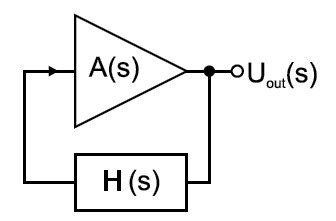
\includegraphics[width=1.0\textwidth]{images/Blockdiagramm_Oszillator}
	  %\subcaption*{Blockdiagramm eines Oszillators}
	% \label{Text}
	\end{minipage}
	\begin{minipage}{0.4\textwidth}
	  \begin{equation*}
        \text{\textbullet }A_cl(s) =\frac{A_(s)}{1-A(s) \cdot H(s)} = \frac{A(s)}{1-T(s)}
      \end{equation*}
      \begin{compactitem}
        \item Schleifenverstärkung: $T(s)$
        \item Für die Oszillations- oder Schwingbedingung gilt: $T(s)=1$
        \item Für das Anschwingen gilt: $T(s)>1$
      \end{compactitem}
	\end{minipage}
\end{figure}
\raggedright
Die Schwingbedingung ist im Normalfall für genau eine Kreisfrequenz $\omega _0$ erfüllt. Man       spricht von Amplituden- und Phasenbedingung, die gleichzeitig bei $\omega _0$ efüllt sein müssen.

\FloatBarrier
\subsubsection{Amplitudenstabilisierung}
Die Schleifenverstärkung ist eine Funktion der Signalamplitude (nichtlinearer Effekt). Für anwachsenden Amplitude wird die Verstärkung kleiner. 
\begin{figure}[h!]
	% minipage mit (Blind-)Text
	\begin{minipage}{0.4\textwidth} 
	  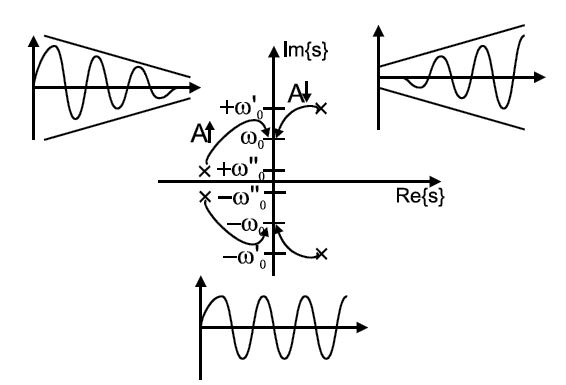
\includegraphics[width=0.9\textwidth]{images/Pollage_Regelung}
	  %\subcaption*{Regelung der Pollage durch amplitudenabhängige Vertärkung}
	\end{minipage}
	\begin{minipage}{0.5\textwidth}
      \begin{compactenum}
        \item Anfangszustand: $T(s)=1$ (Pol befindet sich in rechter s-Halbene)
        \item Signalamplitude steigt exponentiell an.
        \item dadurch wird $T(s)$ reduziert
        \item dadurch werden Pole nach imag.-Achse verschoben (grenzstabil)
        \item falls Pol in inke s-Halbebene gelangt geschiet das umgekehrte
        \item dadurch werden Pole auf Achse gehalten
      \end{compactenum}
	\end{minipage}
\end{figure}

\FloatBarrier
\subsection{Abgestimmte Oszillatoren}
\subsubsection{LC-Oszillatoren}
\begin{figure}[h!]
	% minipage mit (Blind-)Text
	\begin{minipage}{0.3\textwidth} 
	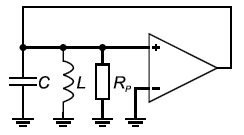
\includegraphics[width=1\textwidth]{images/LC-Oszillator}
	%\subcaption*{Regelung der Pollage durch amplitudenabhängige Vertärkung}
	\end{minipage}
	\begin{minipage}{0.6\textwidth}
      \begin{compactitem}
        \item Trankonduktanz-Verstärker liefert einen zur Eingangsspannung proportionalen Strom
        \item Rückkopplungsnetzwerk: LC-Resonator (Prinzip gilt auch für Serieresonator) 
        \item Schwingbedingung ist bei Resonanzfrequenz des Schwingkreises erfüllt.
        \item höhere Oszillationsfrequenzen möglich als mit RC-Netzwerk
        \item Einsatzgebiet: 1-10 MHz
      \end{compactitem}
       \begin{equation*} 
        \begin{split} 
          \omega_0=\frac{1}{\sqrt{LC}}
        \end{split} 
      \end{equation*}
	\end{minipage}
\end{figure}

\FloatBarrier
\newpage
\subsubsection{Colpitts-Ozsillator}
\begin{figure}[h!]
	% minipage mit (Blind-)Text
	\begin{minipage}{0.3\textwidth} 
	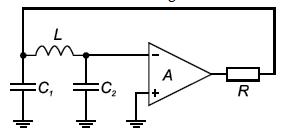
\includegraphics[width=1.1\textwidth]{images/Colpitts-Oszillator}
	\end{minipage}
	\begin{minipage}{0.6\textwidth}
      \begin{compactitem}
        \item Rückkopplungsnetzwerk: $\pi$-Netzwerk\\
      \end{compactitem}
      \begin{equation*} 
        \begin{split} 
           &T(s) = \frac{-A}{1+sR(C_1+C_2)+s^2LC_2+s^3RLC_1C_2}\\
           &\omega _0 = \frac{1}{\sqrt{L\frac{C_1 C_2}{C_1+C_2}}}\\
           &A =\frac{C_2}{C_1} \quad \quad \text{beim Anschwingen gilt:} \quad \quad A \geq\frac{C_2}{C_1} \\
           &\text{(A = Amplitude)} \\
        \end{split} 
      \end{equation*}
	\end{minipage}
\end{figure}

\FloatBarrier
\subsubsection{Quarz-Oszillator}
\begin{figure}[h!]
	% minipage mit (Blind-)Text
	\begin{minipage}{0.3\textwidth} 
	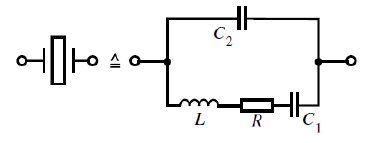
\includegraphics[width=1\textwidth]{images/Ersatzschaltbild_Schwingquarz}
	%\subcaption*{Regelung der Pollage durch amplitudenabhängige Vertärkung}
	\end{minipage}
	\begin{minipage}{0.6\textwidth}
	   Durch anlegen eine Wechselspannung an den Quarz, erhält man eine (bwz. mehrere) Resonsanzfrequenz(en).
       Eigenschaften von Schwingkreisen mit Quarz:
      \begin{compactitem}
        \item sehr temperaturstabil
        \item hohe Güte
        \item hohe Stabilität
        \item Typische Fehlertoleranz ($\frac{\Delta f}{f}$): +/- 20ppm (steigt jedoch quadratisch mit der Abweichung von der optimalen Temperatur (bei Uhrenquarz 25$^\circ$C)) $\rightarrow$ $\quad-0.04ppm/^\circ \text{C}^2$ (typ)\\
        $\frac{\Delta f}{f}=10^(-(^6))...10^(-^(1^(0)))=$
        \item Anschwingbedingung: $g_m \geq R_s\cdot4\omega_0^2C_0 ^2+\frac{4}{R_p}+\frac{1}{R_0}$
        \begin{compactitem}
          \item Es gilt: $ C_0 = C_p+C_1C_2/(C_1+C2)$
        \end{compactitem} 
      \end{compactitem} 
	\end{minipage}
	% minipage mit (Blind-)Text
	\begin{minipage}{0.3\textwidth} 
	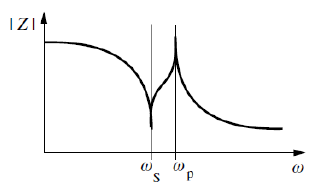
\includegraphics[width=1.0\textwidth]{images/Impedanz(Frequenz)_Schwingquarz}
	%\subcaption*{Regelung der Pollage durch amplitudenabhängige Vertärkung}
	\end{minipage}
	\begin{minipage}{0.6\textwidth}
      %\raggedright
      \vspace{0.5cm}
      Bei der Impedanz eines Schwingquarzes sieht man zwei wesentliche Eigenschaften:
      \begin{compactitem}
        \item zwei Resonanzfrequenzen: Serien- $(Im\{Z(\omega)\}=0)$ und Prallelresonanz $(Im\{Z(\omega)\}=\infty)$
        \item Impedanz ist weitgehend kapazitiv. Induktiv im Bereich:\\ $(\omega_s < \omega < \omega_p)$\\\\ 
      \end{compactitem}
      \begin{equation*} 
        \begin{split} 
         & Z (\omega)=\frac{s^2+\omega _s ^2}{sC_p(s^2+\omega_p ^2)} \quad \text{für } Z(s) = jX(\omega): \quad X(\omega)=-\frac{1}{\omega C_p}\cdot \frac{\omega^2-\omega_s ^2}{\omega^2-\omega_p ^2}\\
        \end{split} 
      \end{equation*}
	\end{minipage}
\end{figure}

\FloatBarrier
\subsection{Nichtabgestimmte Oszillatoren}

\FloatBarrier
\subsubsection{Ringozsillator}
Beim Ringoszillator wird eine ungerade Anzahl Inverter aneinander gereit. Die Frequenz ensteht durch die totale Verzögerung, welche sich aus den einzelnen Verzögerungen der Inverter ergibt.
\begin{figure}[h!]
	\begin{minipage}{0.4\textwidth} 
	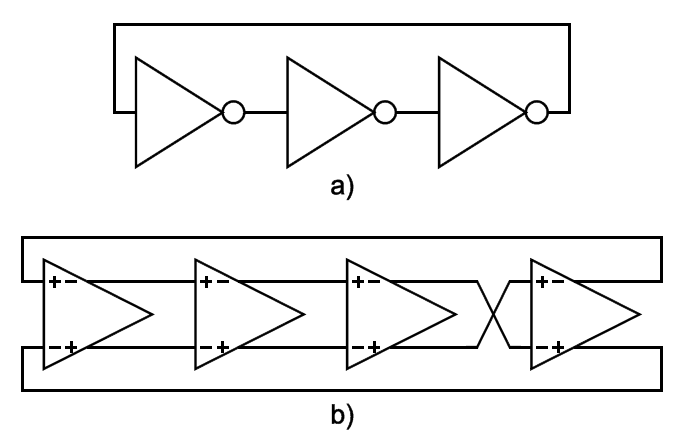
\includegraphics[width=0.8\textwidth]{images/Ring_Osc}
	\subcaption*{Ringoszillator mit a) CMOS-Invertern und b) differentiellen Invertern}
	\begin{equation*} 
        \begin{split} 
          f_{osc} =\frac{1}{2n\cdot t_g} \quad \quad \Delta\varphi =\frac{180^\circ}{2n}   
        \end{split} 
      \end{equation*}
	\end{minipage}
	\begin{minipage}{0.5\textwidth}
	  \begin{compactitem}
        \item Vorteil:
        \begin{compactitem}
           \item hohe $f_{osc}$ 
        \end{compactitem}
        \item Nachteile:
        \begin{compactitem}
           \item $f_{osc}$ ungenau
        \end{compactitem}
        \item Einsatz:
        \begin{compactitem}
           \item Prozesscharakterisierung
           \item Als gesteuerte Oszillatoren in PLL's
        \end{compactitem}
        \item Verzögerung ist Abhängig von der Versorungsspannung
        \item Verzögerung erhöht sich, wenn der Ausgang kapazitiv belastet wird (\"fan-out\")
        \item $n$: Anzahl Inverter
        \item $t_g$: Verzögerung pro Inverter
        \item $\Delta\varphi$: Phansenverschiebung
      \end{compactitem}
	\end{minipage}
\end{figure}

\subsubsection{Multivibrator-Oszillatoren}
Beim Multivibrator wird der Verstärker durch einen Schmitt-Trigger (Komperator mit Hysterese) ersetzt. Als Frequenzbestimmendes Element wird ein RC-Netzwerk verwendet. Die Hysteresefunktion lässt sich dann ausnutzen, um einen Oszillator zu entwerfen. Das RC-Netzwerk als Rückkopplung dient als Tiefpass welcher eine grobe Annäherung eines Integrator darstellt.
\begin{figure}[h!]
	% minipage mit (Blind-)Text
	\begin{minipage}{0.3\textwidth} 
	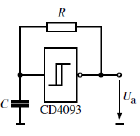
\includegraphics[width=0.7\textwidth]{images/Multivibrator_Komp}
	%\subcaption*{Regelung der Pollage durch amplitudenabhängige Vertärkung}
	\end{minipage}
	\begin{minipage}{0.6\textwidth}
      \begin{compactitem}
        \item max. Komperator Ausgangsspannung:\quad $L_+=V_+$
        \item min. Komperator Ausgnagsspannung:\quad $L_-=V_-$
        \item obere Umschaltschwelle: \quad $V_{TH}=\beta\cdot L_+$
        \item untere Umschaltschwelle: \quad $V_{TL}=\beta\cdot L_-$
        \item Teilungsfaktor: $\beta$\\
       \end{compactitem}
      \begin{equation*} 
        \begin{split} 
          &f_{osc}=\frac{1}{T} \quad \text{mit} \quad T=\tau \cdot ln \frac{(\beta L_- - L_+)(\beta L_+ - L_-)}{(\beta L_+ - L_+)(\beta L_- - L_-)}\\
          & \text{für} \quad   L_+=L_-: \quad  T=2\tau \cdot ln\frac{\beta+1}{\beta-1}\\
        \end{split} 
      \end{equation*}
	\end{minipage}
\end{figure}

\FloatBarrier
\paragraph{Geschalteter Oszillator LM555}
Der LM555 ist ein fertiger IC welcher  mit einem Schmitt-Trigger und dessen Hysterese und exterenen RC-Beschaltung arbeiteite.
\begin{figure}[h!]
	\begin{minipage}{0.5\textwidth} 
	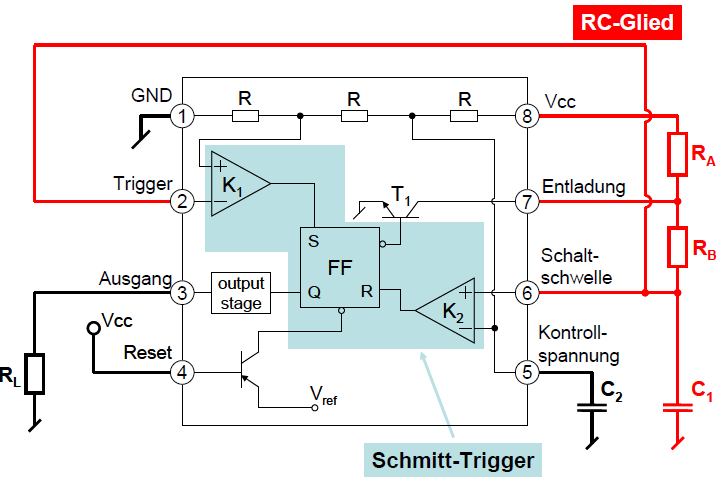
\includegraphics[width=0.9\textwidth]{images/LM555}
	%\subcaption*{Regelung der Pollage durch amplitudenabhängige Vertärkung}
	\end{minipage}
	\begin{minipage}{0.4\textwidth}
	  \begin{compactitem}
        \item Vorteil:
        \begin{compactitem}
           \item $f_{osc}$ ist nur von $R_a, R_B, C_1$ abhängig, nicht von der  Betriebsspannung
        \end{compactitem}
        \item Nachteile:
        \begin{compactitem}
           \item kleine $f_{osc}$
           \item Duty Cycle ist durch unterschiedliche Auf- und Entladezeiten normalerweise asymmetrisch.\\\
        \end{compactitem}
      \end{compactitem}
      \begin{listliketab}
    \begin{tabular}{Llll}
           & Ladezeit:             & $t_1=0.693\cdot(R_A+R_B)C$    \\
           & Entladezeit:          & $t_2=0.693\cdot R_B \cdot C$   \\
           &  Frequenz:             & $f=\frac{1}{T}=\frac{1.44}{(R_A+2\cdot R_B)C}$    \\
    \end{tabular}
\end{listliketab}
	\end{minipage}
\end{figure}

\FloatBarrier
\subsection{Spannungsgesteuerte Oszillatoren (VCO)}
Das Ziel ist es, bekannte Oszillatortopologien so zu nutzen, dass man sie mit einer Spannung oder einem Strom steuern kann. Dafür gibt es folgende Methoden (Siehe Beispiele ab S.6-20 in Skript).

\FloatBarrier
\subsubsection{FET im Anlaufgebiet}
FET's weisen im Anlaufgebiet lineare Anstiege auf, wodurch sie in diesem Bereich als steuerbare Wiederstände eingesetzt werden können.

\FloatBarrier
\subsubsection{Binär geschaltete Elemente}
Da der lineare Werterbereich eines FET's nicht sehr gross ist, werden sie oft als Schalter gebrucht. Dabei wird ein Netzwerk mit R,L,C aufgebaut welche durch die FET's je nach wunsch dazugeschalten werden können. Die FET's nhemen also die Zustände $"$on$"$ oder $"$off$"$ ein. Es handelt sich um eine digitale Ansteuerung. Oft werden C's parallet geschlten, da man diese dann addieren kann und man so mit einem Binärwort gut ansteuern kann. VCO's dessen Frequenz sich mit einem Binärwort in diskreten Schritten einstellen lassen, nennt man $"$Digital Controlled Oscillator (DCO)$"$.

\FloatBarrier
\subsubsection{Diode im Sperrbereich}
Wenn man eine Diode im Sperrbereich betreibt, entsteht eine Sperrschichtkapazität. Diese ist von der DC-Sperrspannung $V_SP$ abhängig. Man hat also einen spannungsgesteuerten Kondensator, den man in einem Schwingkreis einsetzen kann.
\begin{equation*} 
  C_D(V_{SP})=\frac{C_0}{(1+\frac{V_{SP}}{\Phi})^m}
\end{equation*)

\FloatBarrier
\subsubsection{Referenzspannung beim Multivibrator (LM555)}
Durch Veränderung der Schaltschwelle eines Multivibrators lässt sich die Auf- und Entladezeit des Fre-quenz bestimmenden Kondensators variieren. Leider wird durch Manipulation der Schaltschwelle beim Schmitt-Trigger nur die Dauer einer Halbperiode beein-flusst, so dass die Frequenzvariation nur zum "Preis" einer Tastverhältnisvariation erhältlich ist.

\FloatBarrier
\subsubsection{Delay-Interpolation}
\begin{figure}[h!]
	\begin{minipage}{0.25\textwidth} 
      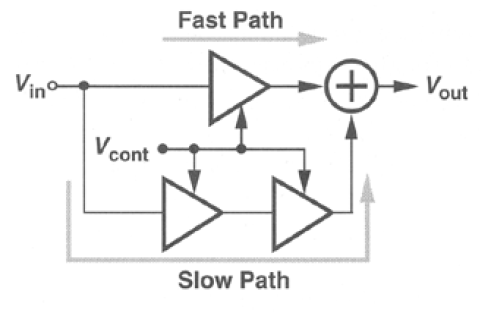
\includegraphics[width=1\textwidth]{images/Fast_Path}
    \end{minipage}
    \begin{minipage}{0.75\textwidth} 
       Bei Ringoszillatoren kann bei differenziellen Invertern die effektive Anzahl Inverter durch Ändern des Schaltstromes zwischen zwei Extremen geändert werden.
       \begin{equation*} 
         f_{min} =\frac{1}{2n_{max}\cdot t_g} \quad \text{und} \quad f_{max} =\frac{1}{2n_{min}\cdot t_g}  
       \end{equation*}
    \end{minipage}
\end{figure}
\raggedright
\section {Phasenregelkreis PLL}
Anwdungsbeispiele von PLL's sind: \textbf{Frequenzsynthese} (Höhere Frequenz am Ausgang als am Eingang), \textbf{Kohärenter Empfang/Trägerrückgewinnung}, \textbf{Frequenzmodulation/Demodulation}.  PLL's lassen sich wie folgt klassifizieren:\\
\begin{compactenum}
    \item \textbf{Vollständig analoge PLL}: Phasendetektor ist analoger Multipliziere, Schleienfilter sowie VCO sind analoge Schaltungsblöcke. Alle Signale zeit-und amplitudenkontinuierlich
    \item \textbf{"Klassischer" digitaler PLL}: Phasendetektor ist digital (Ausgang: diskrete Zustände), der Rest ist analog.
    \item \textbf{Ladungspumpen-PLL ("Charge Pump")}: "Ladungspumpe ist eine Spezielle Art des Schleifenfilters. Ansteuerung der Schalter durch  digitalen Phasendetektor.
    \item \textbf{Volldigitaler PLL (ADPLL)}: Alles wird digital realisiert. Alle Signale können nur diskrete Werte aufnehmen.
    \item \textbf{Software PLL}: Simulation auf einem Computer
\end{compactenum}

\subsection{Grundlagen}
\begin{figure}[h!]
	\begin{minipage}{0.25\textwidth} 
       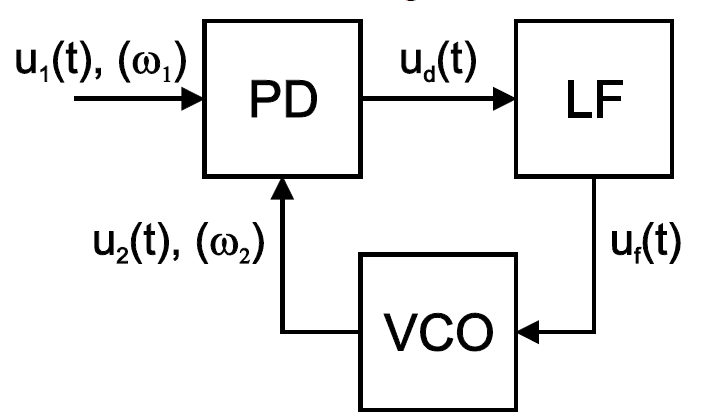
\includegraphics[width=0.8\textwidth]{images/Prinzip_PLL}\\
	\end{minipage}
	\begin{minipage}{0.75\textwidth}
	   Ein PLL ist ein Regelsystem, für die Phase $\varphi_1(t)$ und $\varphi_2(t)$. Das Ziel ist es, die Phase $\varphi_2(t)$ des  VCO's $\varphi_1(t)$ bis auf einen allfälligen (konstanten) Phasenfehler $\Delta \varphi_0$ nachzuregeln.\\
       Weil: $\varphi _1(t\to \infty ) - \varphi_2(t \to \infty)= \Delta \varphi = const$ und somit $\Delta \omega = \frac{d}{dt}\Delta \varphi_0 = 0$ ist, kommt man zum Schluss, dass für die Frequenzen $\omega_1 = \omega_2$ gelten muss.
	\end{minipage}

    \begin{minipage}{0.4\textwidth} 
       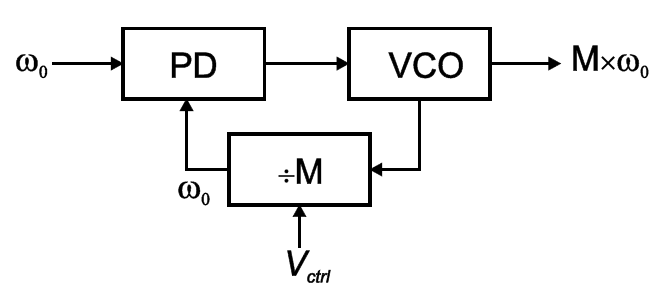
\includegraphics[width=0.9\textwidth]{images/Hohe_Frequ}\\
    \end{minipage}
    \begin{minipage}{0.6\textwidth}
      Vergleicht man das Referenzsignal mit einer durch einen Faktor M geteilten Teil des Oszillatorsignals, ist die Frequenz des Ausgangssignals um den Faktor M grösser als die des Eingangssignals. Wenn $M$ steuerbar ist, lassen sich exakte Vielfache der Frequenz $\omega0$ erzeugen. Lässt sich ein rationales Teilerverhältnis N/M einstellen, spricht man von einer "Fractional-N PLL". Mit speziellen Techniken kann man mit einem Fractional-N PLL kontinuierlich einstellbare Frequenzbereiche erzielen.
    \end{minipage}
\end{figure}

\subsection{VCO} 
\begin{figure}[h!]
	\begin{minipage}{0.25\textwidth} 
       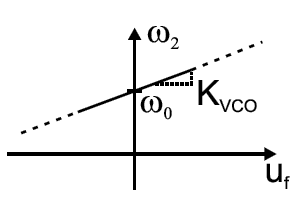
\includegraphics[width=0.7\textwidth]{images/K_VCO}
	\end{minipage}
	\begin{minipage}{0.75\textwidth}
	Aufgabe: Generierung einer Frequenz in Funktion einer Spannung
	   \begin{equation*}
         \begin{split}
            &\omega_2 = \omega_0+K_{VCO}\cdot u_f(t) \quad \quad (K_{VCO}=\text{VCO-Verstärkung})  \\
            &\varphi_2(t) =\int \limits_{t_0}^{t} \omega_2 \ d\tau =\int \limits_{t_0}^{t} \omega _0 + K_{VCO}\cdot u_f (\tau)\ d \tau =\omega_0 t + K_{VCO} \int \limits_{}^{} u_f(\tau) d\tau +\varphi_{20} \\
         \end{split}
        \end{equation*}
	\end{minipage}
\end{figure}

\subsection{Phasendetektor (PD)}
\begin{figure}[h!]
	\begin{minipage}{0.25\textwidth} 
       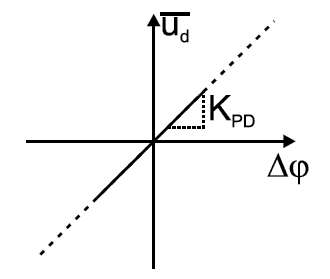
\includegraphics[width=0.7\textwidth]{images/Phasen_Detekt}
    \vspace{0.2cm}
	\end{minipage}
	\begin{minipage}{0.75\textwidth}
	   Aufgabe: Differenzbildner für die Phasensignale. Die mittlere Ausgangsspannung ist: 
	   \begin{equation*}
         \begin{split}
            \overline{u_d}=K_{PD}\cdot \Delta \varphi
         \end{split}
        \end{equation*}
        In der Praxis werden verschiedene Elemente eingesetzt: ($V_0$: max. Wert von $\overline{u_d}$)
	\end{minipage}
\end{figure}

\begin{figure}[h!]
	\begin{minipage}{0.1\textwidth}
        \begin{tabular}{|c|c|c|c|}
          \hline
          Analoger Multipplizierer               & EXOR-Gatter                      & Flankengetriggertes JK-FF                            & Phasen-Frequenzdetektor (PFD)\\
          \hline \hline
          $K_{PD}=\frac{U_1 U_2}{2}\cdot \Delta$ & $K_{PD}=\frac{V_{0}}{\pi}$       & $K_{PD}=\frac{V_{0}}{\pi}=\frac{V_{DD}}{2\pi}$       & $K_{PD}=\frac{V_{0}}{2\pi}=\frac{V_{DD}}{4\pi}$ \\
          \hline
          für $\varphi \to 0 \ (<< 1 rad)$        & für $\Delta\varphi \in [0,\pi]$  & für $\Delta\varphi \in [-\pi,\pi]$                   & für $\Delta\varphi \in [-2\pi,2\pi]$ \\    
          (nichtlinear)                          & Abhängig von                     & nicht abhängig von                                   & 3 Zustände!\\
                                                 & Tastverhältnis!                  & Tastverhältnis!                                      &\\
          \hline
        \end{tabular}
	\end{minipage}
\end{figure}

\FloatBarrier
\subsection{Schleifenfilter}
Aufgabe: Mitteln des PD-Signals (TP-Charakteristik). Dafür gibt es folgenden Methoden:
\begin{figure}[h!]
\begin{minipage}{0.1\textwidth}
        \begin{tabular}{|c|c|c|c|}
          \hline
          Loopfilter mit Charge-Pump *                            & EXOR-Gatter                       & passives Lag-Filter                                   & aktives Lag-Filter\\
          \hline \hline
          $H_{s}=\frac{I{pump}}{2 \cdot \pi \cdot C_p \cdot s}$   & $H_{s}=\frac{1}{1+s\tau}$         & $H_{s}=\frac{1+s\tau _2}{1+s(\tau _1 +\tau _2)}$      & $H_{s}=\frac{1+s\tau _2}{1\tau _1 }$  \\
          \hline
          +1: C aufladen                                          & einfach, oft ungenügend           &                                                       &\\    
          0: Wert behalten                                        & zusätzlich einen Pol              &                                                       & \\
          -1: C entladen                                          & $\to$ evt. Dämpfung zu klein      &                                                       &  \\
          \hline
        \end{tabular}
	\end{minipage}
\end{figure}
\FloatBarrier
* (für PFD) 

\FloatBarrier
\subsection{Linearisierung}
\begin{figure}[h!]
	\begin{minipage}{0.3\textwidth} 
       \includegraphics[width=1\textwidth]{images/linear_PLL}
	\end{minipage}
	\begin{minipage}{0.7\textwidth} 
       \begin{compactitem}
          \item Linearisierung gilt für eingerasteteten PLL ($\omega_1 = \omega_2$) und leichte Abweichung der Ruhelage
          \item lineare Systeme können mit Laplace-Transformation analysiert werden.
       \end{compactitem}
	\end{minipage}
\end{figure}

\FloatBarrier
\subsection{Eigenschaften der PLL im eingerasteten Zustand}
\begin{figure}[h!]
	\begin{minipage}{0.5\textwidth} 
       \includegraphics[width=1\textwidth]{images/PLL_Stabilitaet}
	\end{minipage}
	\begin{minipage}{0.5\textwidth} 
       \begin{compactitem}
          \item Stabilität ist wie bei anderen Regelkreisen wichtig. Sonst rastet PLL nicht ein.
          \item Nullstelle bei $s=\frac{1}{\tau_2}$ muss zu niedrigen Frequenzen verschoben werden, dass System stabil ist.
       \end{compactitem}
	\end{minipage}
\end{figure}

%\begin{figure}[h!]
       \begin{compactitem}
          \item \textbf{Haltebereich (hold range)} $\Delta \omega_H = V_{PD,max}\cdot H(0)\cdot K_{VCO}$: Ist der PLL eingerastet, so rastet er innerhalb des Haltebereichs nicht aus, solange es sich um statische (sehr langsame) Frequenzveränderungen handelt. 
          \item \textbf{Einrastbereich (pull-in range)} $\Delta \omega_{P}$: In diesem Bereich von Frequenzdifferenzen schafft es der PLL, wieder einzurasten. Der Einrastvorgang ist sehr langsam.
          \item \textbf{Ausrastbereich (pull-out range)} $\Delta \omega_{PO}$: Ist eine Frequenzschritt am Eingang der PLL grösser als ΔωPO, dann rastet der PLL aus.
          \item \textbf{Einrastbereich (lock-in range)} $\Delta \omega_{L} \approx 2 \zeta \omega_n$: Bei Frequenzveränderungen, die kleiner sind als ΔωL bleibt der PLL eingerastet. Das sollte der normale Arbeitsbereich eines PLLs sein. Es ist auch die maximale Frequenz, bei der das sofortige Einrasten (lock-in) möglich ist. ($\zeta:$ Dämpfung, $\omega_n$ = natürliche Frequenz.
          \item \textbf{Einrastzeit(lock-in time)} $T_{L} \approx \frac{2\pi}{\omega _n}$: Es ist die Zeit, für das Erreichen des eingerasteten Zustands 
        \end{compactitem}}
%\end{figure}

\FloatBarrier
\subsection{ADPLL (All Digital PLL)}
\begin{figure}[h!]
	\begin{minipage}{0.45\textwidth} 
       \includegraphics[width=1\textwidth]{images/ADPLL}
         \subcaption*{ADPLL}
	\end{minipage}
	\begin{minipage}{0.45\textwidth} 
       \includegraphics[width=1.1\textwidth]{images/linear_ADPLL}
         \subcaption*{Linearisierung ADPLL}
	\end{minipage}
\end{figure}

\begin{multicols}{2}
    \subsubsection{Phasendetektor}
    \begin{compactitem}
        \item \textbf{XOR}  
         \item \textbf{JK-FlipFlop} 
         \item \textbf{FF-Counter} $N$ von $0$ bis $\frac{T_{per}}{T_{clk}}$
         \item \textbf{Nyquist Rate Phase Detector}: Analoger Multiplizierer wird mit ADC und digitaler Multiplikation realisiert.
         \item \textbf{Zero-Crossing Phase Detector)}: Abtastung des Eingagssignals beim Nulldurchgang vom Feedback-Loop
         \item \textbf{Hilbert Transform Phase Detector}
         \item \textbf{Digital-Averaging Phase Detector}
    \end{compactitem}
    
    \subsubsection{Loop-Filter}
    \begin{compactitem}
         \item \textbf{\boldmath$N$ before \boldmath$M$ Loop Filter}  
         \item \textbf{UP/DOWN Counter Loop Filter} 
         \item \textbf{K Counter Loop Filter} 
         \item \textbf{Loop Filter mit \boldmath$N$-bit Parallel Input Signal}
    \end{compactitem}
    
    \subsubsection{Digital-kontrollierbarer Oszillator DCO}
    Realisierung (Programmierbare Frequenzteiler, spezielle Teiler):
    \begin{compactitem}
         \item \textbf{Programmierbarer Frequenzteiler}  
         \item \textbf{ID Counter} 
    \end{compactitem}
    Anwendungen: Skript S.7-11 (ADPLL)
\end{multicols}

\section{Sigma-Delta Wandler}

\subsection{Einführung}
Sigma-Delta Wandler sind überabtastende Wandler, sie verwenden also Abtastfrequenzen, die wesentlich höher sind als die Signalfrequenzen. Für hohe Auflösungen und im Bereich bis 100kSamples werden heute mehrheitlich Sigma-Delta-Wandler eingesetzt.
\subsubsection{Überabgetastete ADCs}
Überabtastung = $f_{s} >> f_{Nyquist}$\ \ \ \ \ \ \ OSR (Oversampling ratio) = Überabtastungsrate (fs / fNyquist)\\
Durch die höhere Abtastfrequenz \textbf{reduziert sich die Rauschleistung} im Signalbandbereich pro Verdoppelung der OSR um 3dB. Die quantisierten Werte mit Frequenz fs werden dezimiert, mit Tiefpassfilter resp. Mittelwertbildner gefiltert: Man erhält so genauere Werte mit Frequenz fNyquist.
\begin{minipage}{0.40\textwidth}
    \includegraphics[width=1.0\textwidth]{images/Prinzipschema}
\end{minipage}
\hfill
\begin{minipage}{0.55\textwidth}
    \begin{compactitem}
        \item Rauschleistungsdichte im Basisband wird durch Überabtastung reduziert
        \item Quantisierer mit reduzierter Auflösung
        \item Dezimierung (Mittelwertbildung) erhöht Auflösung
        \item Einfacheres Anti-Aliasing Filter
    \end{compactitem}
\end{minipage}
\subsubsection{Prinzip der Sigma-Delta-Wandler}
\begin{minipage}{0.40\textwidth}
    \includegraphics[width=1.0\textwidth]{images/Prinzipschema2}
\end{minipage}
\hfill
\begin{minipage}{0.55\textwidth}
    \begin{compactitem}
        \item Hohe Überabtastung $\rightarrow$ SNR-Gewinn von 3dB pro Oktave
        \item Durch negative Rückkoppelung wird Quantisierungsrauschen gefiltert und aus Signalfrequenzbereich entfernt $\rightarrow$ Noise shaping
        \item Integrator hat eine sehr grosse Verstärkung bei niedrigen Frequenzen $\rightarrow$ Hoher Loop-Gain
    \end{compactitem}
\end{minipage}
\subsubsection{Highlights der Sigma-Delta-Wandler}
\begin{minipage}{0.55\textwidth}
    \begin{compactitem}
        \item kleiner Analogteil, wenig Drift und kleine Temperaturabhängigkeit
        \item Monotone Funktion
        \item Linear
        \item Brauchen keine Sample-Hold
    \end{compactitem}
\end{minipage}
\hfill
\begin{minipage}{0.40\textwidth}
    \begin{compactitem}
        \item Einfache Anti-Aliasing-Filter
        \item Aufwändige Digitalfilter (können aber beispielsweise Netzbrumm filtern)
        \item Relativ billig
        \item Mit einem Bandpass-ADC sind auch relativ hohe Frequenzen verarbeitbar
    \end{compactitem}
\end{minipage}

\subsection{Aufbau von Sigma-Delta-Wandlern}
\begin{minipage}{0.55\textwidth}
    \includegraphics[width=1.0\textwidth]{images/AufbauSigmaDeltaWandler}
\end{minipage}
\hfill
\begin{minipage}{0.40\textwidth}
    \begin{compactitem}
        \item Analoger TP dient als Anti-Aliasing-Filter
        \item Der Modulator (wird sehr hoch getaktet) wandelt das analoge Signal in einen digitalen Datenstrom (mit Frequenz fs) um
        \item Datenstrom wird mit digitalem TP gefiltert und durch Dezimierung auf fNyquist reduziert 
    \end{compactitem}
\end{minipage}

\subsection{Sigma-Delta-Modulatoren}
\begin{minipage}{0.55\textwidth}
    \includegraphics[width=1.0\textwidth]{images/AufbauSigmaDeltaModulator}
    \begin{compactitem}
        \item Vom Eingangssignal x(t) wird die Ausgangsspannung von einem DAC subtrahiert
        \item Dieses Differenz-Signal wird mit einem Filter (bei Modulatoren 1. Ordnung ein Integrator $\rightarrow$ sehr grosse Verstärkung bei niedrigen Frequenzen) gefiltert
    \end{compactitem}
\end{minipage}
\hfill
\begin{minipage}{0.40\textwidth}
    \begin{compactitem}
        \item Das Ausgangssignal des Filters wird mit einem ADC in eine zeitdiskrete Datenfolge umgewandelt. \item Der ADC-Wert steuert den DAC, dessen Ausgangsspannung von der Eingangsspannung subtrahiert wird
        \item ADC und DAC sind oft nur ein Bit breit, d.h. es sind Komparatoren resp. Umschalter zwischen zwei Spannungspegeln
    \end{compactitem}
\end{minipage}
\newpage
\subsection{Implementationen von Sigma-Delta-Modulatoren}
\textbf{Integrierender Wandler:}\\
\begin{minipage}{0.55\textwidth}
    \includegraphics[width=1.0\textwidth]{images/IntegrierenderWandler}
\end{minipage}
\hfill
\begin{minipage}{0.40\textwidth}
    \begin{compactitem}
        \item Schaltung für Dual SlopeADC oder Modulator (je nach Schalter-Ansteuerung)
        \item Eingangsbereich Vin von Vrefn bis Vrefp (Ri1=Ri2)
        \item Vrefp und Vrefn symmetrisch um VAGND
    \end{compactitem}
\end{minipage}
\textbf{Charge Balancing Wandler:}\\
\begin{minipage}{0.55\textwidth}
    \includegraphics[width=1.0\textwidth]{images/ChargeBalancing}
\end{minipage}
\hfill
\begin{minipage}{0.40\textwidth}
     $\Delta Q_{Cint} = Cin \cdot Vin \pm Cref \cdot Vref$
    \\\\  $n = N \cdot \frac{Vin \cdot Cin + Vref \cdot Cref}{2 \cdot Vref \cdot Cref}$\\
    \begin{compactitem}
        \item Durch Zählen der "1" im Bitstream (n) kann Vin bestimmt werden: gleitender Mittelwert über N Takte
        \item Je grösser N, desto höher die Auflösung
        \item Kurzer Beobachtungszeitraum: Kleine Auflösung, dafür schnelle Reaktion auf Signalwechsel
        \item Langer Beobachtungszeitraum: Hohe Auflösung, dafür langsamere Reaktion auf Signalwechsel
    \end{compactitem}

\end{minipage}
\textbf{Modulator mit RC-Integrator:}\\
\begin{minipage}{0.55\textwidth}
    \includegraphics[width=1.0\textwidth]{images/SigmaDeltaDualSlope}
\end{minipage}
\hfill
\begin{minipage}{0.40\textwidth}
    \begin{compactitem}
        \item Komparator mit Flip-Flop für Synchronisierung mit CLK 
        \item Vrefp und VRrefn symmetrisch um AGND (+Vref, -Vref)
        \item AGND als virtueller Ground betrachtet (=0V)
        \item Ri1=Ri2, damit Bereich von Vin zw. Vrefp und Vrefn resp. +/-Vref
    \end{compactitem}
\end{minipage}
\begin{minipage}{0.45\textwidth}
    Vin=0V:\\
    \includegraphics[width=1.0\textwidth]{images/Signal1}\\\\
    Vin=-0.5*Vref:\\
    \includegraphics[width=1.0\textwidth]{images/Signal3}
\end{minipage}
\hfill
\begin{minipage}{0.45\textwidth}
    Vin=0.5*Vref:\\
    \includegraphics[width=1.0\textwidth]{images/Signal2}\\\\\\\\
    Vin=-7/8*Vref:\\
    \includegraphics[width=1.0\textwidth]{images/Signal4}
\end{minipage}\\ \ \\ \ \\
\textbf{Pattern Noise:} Kurze repetitive Sequenzen erzeugen hohe Frequenzen, die vom Digitalfilter eliminiert werden. Längere repetitive Sequenzen können innerhalb des Signalfrequenzbandes liegen. Sie können nicht von niederfrequenten Eingangssignalen unterschieden werden und werden damit vom digitalen Filter nicht herausgefiltert.
Dieser Effekt heisst Pattern Noise und ist natürlich in vielen Applikationen inakzeptabel. In der Praxis werden deshalb nur selten Modulatoren 1. Ordnung verwendet. Bei Modulatoren höherer Ordnung entsteht kaum Pattern noise.

\subsection{Modellierung von Sigma-Delta Modulatoren}
\textbf{Laplace-Modell:}\\
\begin{minipage}{0.45\textwidth}
    \includegraphics[width=1.0\textwidth]{images/SigmaDeltaLaplace}
\end{minipage}
\hfill
\begin{minipage}{0.45\textwidth}
   Ausgangssignal:\\ $Y(s)=[X(s)-Y(s)]\cdot \frac{1}{s \cdot T}$\\\\
   Signal-Übertragungsfunktion:\\ $H_{s}(s)=\frac{Y(s)}{X(s)}=\frac{1/(s \cdot T)}{1+1/(s\cdot T)} = \frac{1}{1+s\cdot T}$\\\\
   Rausch-Übertragungsfunktion:\\
   $H_{n}(s)=\frac{Y(s)}{Q(s)}=\frac{1}{1+1/(s\cdot T)} = \frac{s \cdot T}{1+ s \cdot T}$
\end{minipage}\\
Aus diesen beiden Übertragungsfunktionen lässt sich der Vorteil des Sigma-Delta Modulator erkennen. Für die Nutzsignale verhält er sich wie ein Tiefpass, für das Quantisierungsrauschen wie ein Hochpass. Mit anderen Worten: Die Nutzsignale werden nicht verändert, solange ihre Frequenzen nicht grösser sind als die Eckfrequenz des Tiefpasses. Die Sigma-Delta Schlaufe innerhalb des Modulators jedoch schiebt das Quantisierungsrauschen in höhere Frequenzbereiche. Dieses Verschieben wird als "Noise Shaping" bezeichnet.\\ \ \\
\textbf{Zeitdiskretes-Modell:}\\
\begin{minipage}{0.45\textwidth}
    \includegraphics[width=1.0\textwidth]{images/SigmaDeltaZeitdiskretesModell}
\end{minipage}
\hfill
\begin{minipage}{0.45\textwidth}
    Differenzengleichung:\\ $y(n) = x(n-1)+[e(n)-e(n-1)]$\\\\
    Z-Transformation:\\ $Y(z)=z^{-1}\cdot X(z)+E(z)\cdot (1-z^{-1})$\\\\
    Fehlerübertragungsfunktion:\\
    $H_{E1}(z) = E(z) \cdot (1-z^{-1})$\\\\
    Rauschdichte:\\ $N(f)=\sqrt{\frac{2}{fs}}\cdot \frac{q}{12} \cdot 2 \cdot sin(\frac{2 \cdot \pi \cdot f}{fs})$\\\\
    Effektivwert der Rausch-Spannung:\\
    $n0=\frac{q}{\sqrt{12}}\cdot \frac{\pi ^2}{\sqrt{3}}\cdot (\frac{2 \cdot f0}{fs})^\frac{3}{2}$
\end{minipage}


%\subsection{Multibit-Modulatoren}
%Es gibt 2 Möglichkeiten, eine vorgegebene Auflösung zu erreichen: Die Änderung der Überabtastungsrate und der Auflösung des ADC. Für Wandler mit hohen Auflösungsanforderungen (hohes SNR) können Multibit- Modulatoren eingesetzt werden, wenn die Abtastfrequenz nicht erhöht werden kann.

\subsection{Sigma-Delta Modulator 2.Ordnung}
Beim Modulator 2.Ordnung werden ein zweiter Integrator und ein zweiter Summationsknoten addiert.
\begin{minipage}{0.45\textwidth}
    \includegraphics[width=1.0\textwidth]{images/SigmaDelta2Ordnung}
    \includegraphics[width=1.0\textwidth]{images/SigmaDeltaZeitdiskretesModell2}
\end{minipage}
\hfill
\begin{minipage}{0.45\textwidth}
    Differenzengleichung:\\
    $y(n) = x(n-1) + e(n) -2e(n-1) + e(n-2)$\\\\
    Z-Transformation:\\ $Y(z)= z^{-1} \cdot X(z) + E(z) \cdot (1-2\cdot z^{-1} + z^{-2}) = z^{-1} \cdot X(z) + E(z) \cdot (1-z^{-1})^2$\\\\
    Fehlerübertragungsfunktion:\\
    $H_{E2}(z) = E(z) \cdot (1-z^{-1})^2$\\\\
    Effektivwert des Quantisierungsrauschens:\\
    $n0=\frac{q}{\sqrt{12}}\cdot \frac{\pi ^2}{\sqrt{5}}\cdot (\frac{2 \cdot f0}{fs})^\frac{5}{2}$
    
\end{minipage}
\subsection{Modulatoren höherer Ordnung}
\begin{compactitem}
    \item Modulatoren mit Ordnungen \textgreater 2 können instabil werden
    \item Effekt der spektralen Verschiebung des Quantisierungsrauschens wird weiter verstärkt
    \item Noise Shaping funktioniert nicht nur bei tiefen Frequenzen und Tiefpass-Filtern sondern auch mit Bandpass-Filtern $\rightarrow$ Bandpass Sigma-Delta-Wandler
\end{compactitem}

\subsection{Dynamikgewinn durch Sigma-Delta Modulatoren}
Werden die einzelnen Fehlerfunktionen untersucht, so stellt man fest, dass mit jeder Erhöhung der Ordnung eines Sigma-Delta Modulators die Hochpass Funktion kaskadiert wird. Mit jeder Erhöhung der Ordnung steigt der Signalrauschabstand um 6dB pro Oktave an, was dem Anstieg eines Integrators entspricht: $SNR = 10 \cdot log_{10} (\frac{3}{2} \cdot \frac{2M+1}{\pi^{2M}}\cdot OSR^{2M+1})$\ \ \ \ \
$OSR=fs/2f0$ \ \ \ \ \ M = Modulatorordnung\\ 
\textbf{Bei einer Verdoppelung der Abtastrate wird der Dynamikbereich um 9dB oder 1.5 Bit erhöt!}


\section{Piezos und Ultraschall}

\subsection{Grundlagen}
Piezokeramische Bauelemente wandeln mechanische Signale wie Kraft, Druck, Dehnung oder
Beschleunigung in eine elektrische Spannung um oder umgekehrt. Die typischen Resonanzfrequenzen liegen dabei zwischen 40 kHz und 10 MHz. Der piezoelektrische Effekt tritt sowohl in \textbf{einkristallinen Materialien} als auch
in \textbf{polykristallinen ferroelektrischen Keramiken} auf.
\begin{compactitem}
    \item Direkter piezoelektrischer Effekt: Bei Druckeinwirkung (wandelt mech. in elektr. Energie um)
    \item Indirekter piezoelektrischer Effekt: Bei Anlegen einer elektr. Spannung (wandelt elektr. in mech. Energie um)
\end{compactitem}

\subsubsection{Piezoelektrische Kristalle}
\begin{compactitem}
    \item Der wichtigste piezoelektrische Kristall ist die vom Quarz gebildete bis zu 573 ${^\circ}$ C stabile trigonale Kristallstruktur $\alpha$-Quarz. Die wichtigste Anwendung sind Schwingquarze.
    \item Lithiumniobat hat gegenüber Quarz höhere piezoelektrische Konstanten und wird für piezoelektrische Filter und SAW-Bauelemente (engl.: surface acoustic wave, Akustische Oberflächenwelle) verwendet.
\end{compactitem}

\subsubsection{Piezoelektrische Keramik}
Industriell hergestellte Piezoelemente sind zumeist Keramiken. Gegenüber piezoelektrischen Kristallen haben piezoelektrische Keramiken den Vorteil wesentlich höherer piezoelektrischer Koeffizienten. 
\begin{compactitem}
    \item  Bestehen aus synthetischen, anorganischen, ferroelektrischen und polykristallinen Keramikwerkstoffen
    \item Typische Basismaterialien sind modifizierte Blei-Zirkonat-Titanate (PZT) und Blei-Magnesium-Niobate (PMN)
\end{compactitem}
\textbf{Blei-Zirkonat-Titanate (PZT):}
\begin{compactitem}
    \item Unterhalb der Curie-Temperatur $T_{C}$ wird die Gitterstruktur der PZT-Kristallite verzerrt und asymmetrisch. Es entstehen Dipole und die für die Piezotechnologie interessanten rhomboedrischen bzw. tetragonalen Kristallitphasen bilden sich heraus. Die Keramik weist eine spontane Polarisation auf. Oberhalb der Curie-Temperatur verliert eine Piezokeramik ihre piezoelektrischen Eigenschaften.
    \item PZT-Piezokeramik ist in vielen Variationen (spez. Dotierungen z.B. mit Ni-, Bi-, La-Ionen) verfügbar und die am häufigsten verwendete Keramik für Aktor- oder Sensoranwendungen. 
\end{compactitem}

\subsection{Elektrische Ersatzschaltung}
Das elektromechanische Verhalten eines zu Schwingungen angeregten piezoelektrischen Körpers lässt sich mit folgendem elektrischen Ersatzschaltbild darstellen:\\ 
\begin{minipage}{0.5\textwidth}
    \includegraphics[width=1.0\textwidth]{images/Ersatzschaltbild_Piezo}
\end{minipage}
\hfill
\begin{minipage}{0.45\textwidth}
    \textbf{Schwingkreisbeschreibung bei Frequenzen in der nähe der mech. Eigenresonanz:}
    \begin{compactitem}
        \item $C_{0}$ $\rightarrow$  Kapazität des Dielektrikums
        \item Reihenschaltung $C_{1}$, $L_{1}$, $R_{1}$ $\rightarrow$ beschreibt die Änderung
        der mechanischen Eigenschaften wie elastische Deformation, effektive Masse (Trägheit) und mechanische Verluste durch innere Reibung\\
    \end{compactitem}
    $Z1 = s\cdot L1 + \frac{1}{s\cdot C1} + R1$ \ \ \ \ $Z2 = \frac{1}{s\cdot C0}$ \\\\ $\rightarrow$ $Zpiezo = \frac{(s\cdot L1 + \frac{1}{s\cdot C1} + R1)\cdot \frac{1}{s\cdot C0}}{s\cdot L1 + \frac{1}{s\cdot C1} + R1 + \frac{1}{s\cdot C0}} = \frac{C1\cdot L1\cdot s^2 + C1\cdot R1\cdot s + 1}{s\cdot (C0+C1)\cdot (\frac{C0\cdot C1}{C0 + C1}\cdot L1\cdot s^2 + \frac{C0\cdot C1}{C0 + C1}\cdot R1\cdot s + 1)}$
\end{minipage}

\subsection{Piezos als Schallwandler - Buzzer}
%\subsubsection{Grundlagen}
%\textbf{Lautstärke:} Bei 2kHz liegt die Frequenz bei einem Schalldruckpegel von null Dezibel, entsprechend 20 $\mu$ Pa. \ Flüstern $\rightarrow$ ca. 20dB / Konversation $\rightarrow$ ca. 60dB / Bahnunterführung $\rightarrow$ ca. 100dB\\
%\textbf{Tonhöhe:} Infraschall $\rightarrow$ 0Hz - ca. 16Hz / Hörbarer Bereich $\rightarrow$ 16 Hz - ca. 20kHz  / Ultraschall $\rightarrow$ ab ca. 16kHz

\subsubsection{Funktionsweise}
\begin{minipage}{0.5\textwidth}
    \includegraphics[width=0.8\textwidth]{images/Buzzer_Funktionsweise}
\end{minipage}
\hfill
\begin{minipage}{0.45\textwidth}
    \begin{compactitem}
        \item Metallplatte bleibt
        \item Piezo ändert Länge $\rightarrow$ biegt sich durch
        \item Höherer Schalldruck kann durch Gehäuse erzielt werden
    \end{compactitem}
\end{minipage}
\subsubsection{Funktion des Gehäuses}
 Je nach Bauform beeinflusst das Gehäuse die Schalldruckcharakteristik.
 \includegraphics[width=0.8\textwidth]{images/FunktionDesGehaeuses}
\subsubsection{Oszillation}
\includegraphics[width=0.6\textwidth]{images/OszillationBuzzer}

\subsection{Piezos als Schallwandler in
Ultraschall-Anwendungen für
Messtechnik - Transducer}
\subsubsection{Messverfahren}
Ultraschall-Abstands-Messung  \ \ \ \ \ \ Ultraschall-Distanz-Messung\\
\includegraphics[width=0.6\textwidth]{images/Messverfahren}
\subsubsection{Schallausbreitung}
Energie verteilt sich mit der Zeit auf grössere Fläche. Schalldruck $\sim$ 1/Distanz\\ Bsp: Doppelte Distanz $\rightarrow$ Schall-Leistung verteilt sich auf doppelte Fläche $\rightarrow$ halber Schalldruck
\subsubsection{Absorption}
Absorption in dB/m // Faktor 10 in Frequenz $\rightarrow$ Faktor 100 in Absorption // 1MHz: 100dB/m // 100kHz: 1dB/m

\subsection{Anwendung Durchflussmessung}
\begin{minipage}{0.3\textwidth}
    \includegraphics[width=0.8\textwidth]{images/AnwendungDurchflussmessung}   
\end{minipage}
\hfill
\begin{minipage}{0.65\textwidth}
    \begin{compactitem}
        \item Upstream TOF: $t_{BA} = \frac{l}{c-v}$
        \item Downstream TOF: $t_{AB} = \frac{l}{c+v}$
        \item Water velocity: $v = \frac{(t_{BA}-t_{AB})\cdot c^2}{2 \cdot l}$
    \end{compactitem}
\end{minipage}

\subsection{Piezos
in bildgebenden medizinischen
Ultraschall-Anwendungen}

\begin{minipage}{0.3\textwidth}
    \subsubsection{Schall-Leitung im Körper}
    Schall wird vom Gewebe reflektiert. Reflektierendes Signal wird gemessen.\\
    \includegraphics[width=1.0\textwidth]{images/SchallLeitung}\\\\
\end{minipage}
\hfill
\begin{minipage}{0.2\textwidth}
    \subsubsection{Brechung}
    \includegraphics[width=0.4\textwidth]{images/Brechung}\\
    $\frac{sin \theta _{i}}{sin \theta _{t}} = \frac{v1}{v2}$\\\\\\\\\\\\
\end{minipage}
\hfill
\begin{minipage}{0.4\textwidth}
    \subsubsection{Beamforming}
    \begin{compactitem}
        \item Mit Transducer-Arrays kann Strahl ‘geformt’ werden
        \item Positionsabhängige Delays
    \end{compactitem}
    \includegraphics[width=0.6\textwidth]{images/Beamforming1}\\
    \includegraphics[width=0.8\textwidth]{images/Beamforming2}
\end{minipage}
\section {MEMS (Mikro-Elektro-Mechanische-Systeme)}
\begin{compactitem}
    \item Materialen: Silizium, Polymere, Metalle, Keramik
\end{compactitem}


\subsection{Herstellungsverfahren}
\subsubsection{Bulk Micromachining}
\begin{multicols}{2}
    \begin{compactitem}
      \item Selektives Ätzen aus dem Silizium
      \item Ätzmittel: Fluorwasserstoff, Salpetersäure, Essigsäure (korrosiv)
      \item Vorteile:
      \begin{compactitem}
          \item Schnelles, gleichförmiges Verfahren über grosse Waferflächen
          \item Günstig bezüglich Zeit \& Geld
      \end{compactitem}
      \item Nachteile:
      \begin{compactitem}
          \item Keine komplexen Strukturen
          \item Nicht geeignet für Submikrometerbereich (Undercut)
      \end{compactitem}
      \item Anwendung:
      \begin{compactitem}
          \item Drucksensoren
      \end{compactitem}
    \end{compactitem}

    \includegraphics[width=0.54\textwidth]{images/Bulk_Micro}
\end{multicols}



\subsubsection{Surface Micromachining}
	\begin{minipage}{0.4\textwidth}
      \begin{compactitem}
        \item Schichtenaufbau mit Ätzen:
        \begin{compactitem}
            \item Siliziumnitrid $\rightarrow$ Schützt Substrat
            \item Siliziumoxid $\rightarrow$ Opferschicht
            \item Maske auf Siliziumoxid
            \item Polysilizium  $\rightarrow$ Tragende Schicht
            \item Wegätzen der Opferschicht
            \item (Ähnlich IC-Produktion)
        \end{compactitem}
      \end{compactitem}

	  \begin{compactitem}
	    \item Schichtenaufbau mittels Sputtering:
        \begin{compactitem}
            \item Wafer in Vakuumkammer an Anode
            \item Opfermaterial (bspw. Metall) an Kathode
            \item Ionisiertes Gas (Argon) einleiten
            \item Gasionen treffen auf Opfermaterial
            \item Metallatome haften auf Wafer
        \end{compactitem}
      \end{compactitem}  
      \begin{compactitem}
        \item Vorteile:
        \begin{compactitem}
          \item AnisotropischesVerfahren $\rightarrow$ Keine Undercuts
          \item Komplexere Strukturen
        \end{compactitem}
        \item Nachteile:
          \begin{compactitem}
            \item Sputtering $\rightarrow$ Strahlungsschäden
            \item Zeitaufwändiger und teurer
          \end{compactitem}
      \end{compactitem}
    \end{minipage}
    \hfill
    \begin{minipage}{0.5\textwidth}
    \vspace{-0pt}
      \begin{compactitem}
       \item Anwendung:
        \begin{compactitem}
          \item Freiträger, Brücken, Hohlräume
          \item Turbinen, Zahnräder
        \end{compactitem}
      \end{compactitem}
      \includegraphics[width=1\textwidth]{images/Schichtenaufbau}
      \includegraphics[width=1.\textwidth]{images/Sputtering}
	\end{minipage}


\subsection{MEMS Oszillatoren}
	\begin{minipage}{0.4\textwidth}
      \begin{compactitem}
        \item Vorteile:
        \begin{compactitem}
          \item FlexibeleinstellbareFrequenz
          \item Low cost
        \end{compactitem}
        \item Nachteile:
        \begin{compactitem}
          \item Toleranzen sind gross (ca. 10\%) $\rightarrow$ Abgleich nötig $\rightarrow$ PLL 
        \end{compactitem}
         \item Anwendungsfrequenz: 1Hz - 625 MHz bis 6 decimals (ppm)
      \end{compactitem}
    \end{minipage}
    \hfill
    \begin{minipage}{0.5\textwidth}
       \vspace{0pt}
       \includegraphics[width=0.9\textwidth]{images/MEMS_Oszillator}   
    \end{minipage}


\subsection{Grundformeln}
\label{subsec:Grundformeln}
\subsubsection{Mechanik}
	\begin{minipage}{0.3\textwidth}
      \begin{equation*} 
        \begin{split} 
            &\overrightarrow{F}=\overrightarrow{a} \cdot m\\
            &F=k_m \cdot \Delta x  \quad (\text{Federkonstante } K_m)\\
            &\Delta x=\frac{m}{k_m} \cdot a\\
            &F_d \sim \frac{d_x}{dt} \quad (\text{Dämpfungskraft } F_d)\\
            &F(t)=m\cdot \frac{d^2}{dt^2}x(t)+D \cdot \frac{d}{dt}x(t)+k_m \cdot x(t)\\
            &F(s)=(m \cdot s^2 + D \cdot s + k_m)\cdot X(s) \\
            &H{sensor}(s)=\frac{X(s)}{F(s)}=\frac{1}{m\cdot s^2 + D\cdot s + k_m} \\
            &\text{D: Dämpfungskonstante}
        \end{split} 
      \end{equation*}
    \end{minipage}
    \hfill
    \begin{minipage}{0.6\textwidth}
      \vspace{0pt}
      \paragraph{Verglich mit TP 2.Ordnungm}
      \includegraphics[width=1.0\textwidth]{images/Mech_Regel}  
    
      \begin{minipage}{1.0\textwidth}
        \vspace{0pt}
        \hspace{1cm}
        $\omega _0= \sqrt{\frac{k_m}{m}}$   $ \quad \quad Q=\frac{m\cdot  \omega_0}{D}$
        $\quad \quad H_{LP}= \frac{A \cdot \omega_0 ^2}{s^2 +\frac{\omega _0=}{Q}\cdot s + \omega _0 ^2}$
       \end{minipage}
    \end{minipage}
    
\subsubsection{Elektrostatik}

    $C=\frac{Q}{V} \quad \quad \quad E=\frac{1}{2}\cdot C \cdot V^2 \quad \quad \quad F_{es}=\frac{d}{d_x}\cdot E = \frac{1}{2} \cdot \frac{d}{d_x} \cdot C \cdot V^2$
    
\paragraph{Für parallele Platten}
    \begin{minipage}{0.4\textwidth}
    \vspace{-1cm}
    \begin{equation*} 
      \begin{split} 
         &C(x)=\frac{\epsilon_r \cdot \epsilon_0 \cdot A}{x_0 + x} \\
         &F_{es}(x)=\frac{\epsilon_r \cdot \epsilon_0 \cdot A}{2(x_0+x)^2}\cdot V^2 \approx -\frac{A\epsilon_0\epsilon_r V^2}{2x_0^2}+\frac{A\epsilon_0\epsilon_r V^2}{x_0^3}\cdot x 
      \end{split} 
    \end{equation*}
    \end{minipage}
    \hfill
    \begin{minipage}{0.4\textwidth}
      \vspace{0pt}
      \includegraphics[width=0.9\textwidth]{images/Plattenkondens}
    \end{minipage}

\vspace{-0.5cm}
\subsubsection{Elektrostatische Federkonstante}
\vspace{-0.5cm}
    \begin{equation*} 
      \begin{split} 
        &F(t)=m\cdot \frac{d^2}{dt^2}x(t)+D \cdot \frac{d}{dt}x(t)+(k_m- \frac{A\epsilon_0\epsilon_r V^2}{x_0^3})x(t)= -\frac{A\epsilon_0\epsilon_r V^2}{2x_0^2}+F \\
        &k_{eff}=k_m+k_{es}=k_m- \frac{A\epsilon_0\epsilon_r V^2}{x_0^3} \quad \quad \text{(}k_{eff} \quad \text{darf nicht negativ werden und beeinflusst Resonanzfrequenz.)}\\
      \end{split} 
    \end{equation*}

\subsection{Messung Auslenkung}
\begin{minipage}{0.6\textwidth}
  Kleine Auslenkungen können mit zwei Kondensatorplatten gemessen werden (siehe \ref{subsec:Grundformeln}). Für grössere Auslenkungen kann ein System mit konstanter Lasung $Q$ verwendet werden (Charge control). Gesamte Energie im System: \\
    \begin{equation*} 
        \begin{split} 
           &E=\frac{Q^2}{2C}=\frac{(x_0 + x)Q^2}{2A\epsilon_0 \epsilon_r}
        \end{split} 
    \end{equation*}
  Für 2 C: keine Kraft wirkt, wenn kein Strom durch $mid$ fliesst.\\ $\rightarrow$ Spannungsmessung, nicht Ladungsverstärker.
\end{minipage}
\begin{minipage}{0.3\textwidth}
    \vspace{0pt}
    \includegraphics[width=1.2\textwidth]{images/Bewegung_C}
\end{minipage}
\begin{compactitem}
    \item Vorteile: Einfaches Syste
\end{compactitem}
\begin{compactitem}
    \item Nachteile: Auslenkund ist nichtlineare Funktion der Kraft, Messung mit Ladungsverstärkter bewirkt ebenfalls Kraft
\end{compactitem}


\subsubsection{Kamm-Struktur für grössere Auslenkungen, z.B. Gyros}
\begin{minipage}{0.3\textwidth}
\vspace{-0.5cm}
  \begin{equation*}
    \begin{split} 
      &h\text{:       Dicke der Struktur}\\
      &n_{gap}\text{: Anzahl Abstände}\\
      &g\text{:       Abstand}\\
    \end{split} 
  \end{equation*}
\end{minipage}
\begin{minipage}{0.3\textwidth}
\vspace{-0.5cm}
  \begin{equation*} 
    \begin{split} 
      &C=\frac{\epsilon_0 \epsilon_r\cdot n_{gap}(x_0-x)h}{g}\\
      &E=\frac{1}{2}CV^2\\
      &F_{es}=-\frac{\epsilon_0 \epsilon_r \cdot n_{gap} h v^2}{2g}\\
    \end{split} 
  \end{equation*}
\end{minipage}
\begin{minipage}{0.3\textwidth}
    \vspace{-0.7cm}
    \includegraphics[width=1.2\textwidth]{images/Kamm_Strukt}
\end{minipage}

\vspace{-0.5cm}
\subsection{Messung mit Force Feedback}
\begin{minipage}{0.4\textwidth}
  \begin{compactitem}
    \item Ziel: 
    \begin{compactitem}
        \item Masse in Mitte halten
        \item elektrostat. Kraft als Gegenkraft zur mech. Kraft  aufbringen
        \item elektrostat. Kraft wird kontrolliert, ist bekannt $\rightarrow$ Beschleunigung kann berechnet werden.
    \end{compactitem}
  \end{compactitem}
  \begin{compactitem}
    \item Vorteile:  Elektrostatische Kraft ist bekannt $(F\sim V)$, linear
  \end{compactitem}
  \begin{compactitem}
    \item Nachteile: Regelkreis kann instabil werden bei hoher Ordnung
  \end{compactitem}
\end{minipage}
\hfill
\begin{minipage}{0.5\textwidth}
    \vspace{0pt}
    \hspace{-0.7cm}
    \includegraphics[width=1.1\textwidth]{images/Force_Feedback}
\end{minipage}

\subsection{Auswertung von Kapazitäten}
\subsubsection{Auswertung mit Demodulation}
\begin{minipage}{0.3\textwidth}
  Die beiden Kondensatoren werden mit inversen Rechteck-Impulsen angesteuert. Am Ausgang des Verstärkers erhält man dann immer einmal ein pos. und sonst ein neg. Signal. Dieses wird dann mit $\pm 1$ muliipliziert, um ein positives Signal zu erhalten, welches dann noch gefiltert wird, bevor es dann auf einen ADC geht.
\end{minipage}
\hfill
\begin{minipage}{0.6\textwidth}
    \vspace{0pt}
    \hspace{-0.7cm}
    \includegraphics[width=1.0\textwidth]{images/Demodulation}
\end{minipage}

\subsubsection{Ladungsverschiebung und Charge Sensing}
 $V_{out}$ lässt sich für beide gleich berechnen:   $V_{out}=-V_0 \cdot \frac{\Delta C }{C_{int}}\quad \quad \quad C_{int} \approx 2C_0$  (typisch, Gain-Speed Tradeoff)   \\
Nachteil: Elektrostatische Kräfte beeinflussen mech. Verhalten.\\
Vorteil bei Charge-Sensing: Paracitics werden nicht umgeladen, haben daher keinen Einfluss auf Ausgangssignal.
\hfill
\begin{minipage}{0.45\textwidth}
    \vspace{0pt}
    \hspace{-0.7cm}
    \includegraphics[width=1.0\textwidth]{images/Ladungsverschiebung}
\end{minipage}
\hfill
\begin{minipage}{0.45\textwidth}
    \vspace{0pt}
    \includegraphics[width=1.0\textwidth]{images/charge_sensing}
\end{minipage}

\section{Konstanten}
$k = 1,3806505 \cdot 10^{-23} J/K$ \ \ \ \ \ \ \ \ \ \ $\epsilon_0 = 8.8541...\cdot 10^{-12} \frac{As}{Vm}$ \\
$T$ in Kelvin: 273,15 +  $\vartheta$  in $^\circ $C \ \ \ \ \ \
$\mu _0 = 4\pi \cdot 10^{-7} \frac{N}{A^2}=1.2566..\cdot 10^{-7} \frac{N}{A^2}$





\end{document}
